\documentclass[10pt,letterpaper,onecolumn]{article}

\usepackage{adjustbox}
\usepackage[utf8]{inputenc}
\usepackage{titlesec}
\usepackage{tikz}
\usetikzlibrary{patterns, spy}
\setcounter{secnumdepth}{4}
\titleformat{\paragraph}
{\normalfont\normalsize\bfseries}{\theparagraph}{1em}{}
\titlespacing*{\paragraph}
{0pt}{3.25ex plus 1ex minus .2ex}{1.5ex plus .2ex}
\usepackage[cmex10]{amsmath}
\usepackage{subfiles}
\usepackage{caption}
\usepackage{subcaption}
\usepackage{xspace}
\usepackage{graphicx}
\usepackage{csquotes}
\usepackage[hyphens]{url}
\usepackage{xspace}
\usepackage{amssymb}
\usepackage{siunitx}
\sisetup{
  group-separator={,}, 
  group-four-digits=true, 
  binary-units = true,
  table-number-alignment = center,
}
\usepackage[sort&compress, numbers]{natbib}
\usepackage{acronym}
\usepackage[section]{placeins}
\usepackage{pbox}
\usepackage[overload]{textcase}
\usepackage{tabu, booktabs}
\usepackage[hyphens]{url}
\usepackage{algorithm, algpseudocode}
\usepackage[inline]{enumitem}
\setlist[enumerate]{label=(\arabic*), itemjoin={,\ }, itemjoin*={,\ and\ }}
\usepackage{hyphenat}
\usepackage{color}
\usepackage[margin=1in]{geometry} % change default margins

\title{Systematically Providing Descriptive Names for Unit Tests \\ 
[24pt] Ph.D. Dissertation Proposal}
\author{\textbf{Jianwei Wu} \\
{\small Email: wjwcis@udel.edu} \\\\
\\
Department of Computer and Information Sciences \\
University of Delaware \\\\
}
\usepackage[capitalize,sort]{cleveref}
\usepackage{listings}
\lstdefinestyle{custom_java}{
  belowcaptionskip=1\baselineskip,
  basicstyle=\scriptsize,
  captionpos=b,
  breaklines=true,
  xleftmargin=\parindent,
  language=Java,
}
\lstset{
  style=custom_java,
}
\newcommand{\includecode}[2][c]{\lstinputlisting[escapechar=, style=custom_#1]{#2}}

\begin{document}

\maketitle
\thispagestyle{empty} % do not include numeration in cover page
\newpage % separate cover page from content

\tableofcontents
\newpage

\section*{Abstract}
\addcontentsline{toc}{section}{Abstract}
\label{sec:abstract}




\newpage

\section{Introduction}
\label{sec:introduction}

Unit tests are an important artifact that supports the software development process in several ways.
% change done here 
In addition to helping developers ensure the quality of their software by checking for failures~\cite{daka2014survey}, they can also serve as an important source of documentation not only for human developers but also for automated software engineering tools (e.g., recent work on fault localization by \citeauthor{li2019deepfl} uses test name information~\cite{li2019deepfl}).
%
For example, when a test fails, its name can provide the first step towards understanding the purpose of the test and ultimately fixing the cause of the observed failure.
%
Similarly, a test's name can help developers decide whether a test should be left alone, modified, or removed in response to changes in the application under test and whether the test should be included in a regression test suite.


In this work, we believe that test names are \enquote{good} if they are descriptive (e.g, they accurately summarize both the scenario and the expected outcome of the test~\cite{trenk14}, or being unique among its associated test class) and \enquote{bad} if they are not descriptive.
%
This is because descriptive names:
\begin{enumerate*}
\item make it easier to tell if some functionality is not being tested---if a behavior is not mentioned in the name of a test, then the behavior is not being tested
\item help prevent tests that are too large or contain unrelated assertions---if a test cannot be summarized, it likely should be split into multiple tests
\item serve as documentation for the class under test---a class's supported functionality can be identified by reading the names of its tests
\end{enumerate*}~\cite{zhang2015automatically}.


Unfortunately, unit tests often lack descriptive names.
%
For example, an exploratory study by \citeauthor{zhang2015automatically} found that only \SI{9}{\percent} of the \num{213423} test names they considered were complete (i.e., fully described the body of test) while \SI{62}{\percent} were missing some information and \SI{29}{\percent} contained no useful information (e.g., tests named \enquote{test})~\cite{zhang2015automatically}.
%
Poor test names can be due to developers writing non-descriptive or incomplete names.
%
They can also occur due to incomplete code modifications.
%
For example, a developer may modify a test's body but fail to make the corresponding changes to the test's name.
%
Regardless of the cause, non-descriptive test names complicate comprehension tasks and increase the costs and difficulty of software development.


Because non-descriptive names negatively impact software development, there have been several attempts to address this issue.
%
One approach has been to automatically generate names based on implementations (e.g.,~\cite{arcuri2014automated, zhang2015automatically, daka2017generating}).
%
For example, \citeauthor{zhang2015automatically} and \citeauthor{daka2017generating} use static and dynamic analysis, respectively, to extract important expressions from a test's body and natural language processing techniques to transform such expression into test names \cite{zhang2015automatically, daka2017generating}. 
%
While automatically generating names from bodies eliminates the possibility of mismatches between names and bodies the generated names do not always meet with developer approval (e.g., they may not fit with existing naming conventions).
%
Another approach is to help developers improve their existing names by suggesting improvements.
%
For example, \citeauthor{host2009debugging} proposed an approach for Java methods and variables which uses a set of naming rules and related semantics~\cite{host2009debugging}, \citeauthor{li2019deepfl} provided a learning-based approach to locate software faults using test name information \cite{li2019deepfl}, and \citeauthor{allamanis2015suggesting} and \citeauthor{pradel2018deepbugs} use a model-based and a learning-based approach, respectively, to directly suggest better names or find name-based bugs to facilitate improvements~\cite{allamanis2015suggesting, pradel2018deepbugs}.


Judging from the collected results of our empirical studies~\cref{sec:empStudy,sec:test-pattern-section}, different developers often use different naming rationales for writing test names.
%
Many of the test names that were inspected are named after either what makes the test unique from the test body (i.e., the uniqueness of the test) or a summarization of the action, predicate, and scenario of the test body (i.e., the descriptiveness of the test).
%
Therefore, to address the lack of descriptive names in unit tests (i.e., test names that can summarize important parts of the test body or being unique in its test class), I propose two approaches that can both be used to systematically provide descriptive names for unit tests.
%
According to the two major naming rationales of the naming unit tests, our first approach is based on the uniqueness of the test to construct descriptive test names, and the second approach is based on the descriptiveness of the test for the same purpose.
%
The focus of both approaches is to provide descriptive names (i.e., \enquote{good} names) for unit tests.
%
Any test name that is named after the uniqueness or the descriptiveness of the test should be considered as a descriptive test name, which also means a \enquote{good} test name could be constructed after one or more naming rationales depending on the amount of information it needs to contain.


In this proposal, I propose the following research tasks, which will contribute to two approaches that can systematically provide descriptive names for unit tests from two distinct aspects.
%
First, in order to show the evidence that different developers often use different naming rationales to name their tests, an empirical study is conducted as the first step of building the three approaches, and a set of selective codes are also produced as part of the results of the empirical study.
%
Using the results of the empirical study, we found out that most of the inspected tests are indeed named after what makes them unique, and the uniqueness of tests can be identified and utilized for future improvement by a set of top-level and secondary codes, which comes from the selective coding process using basic Java code elements as shown in~\cref{sec:test-pattern-section}.
%
Moreover, different test names are shown to be named after different naming rationales like uniqueness-based or descriptiveness-based.
%
Some tests are named after the uniqueness of the test name and body, while other tests are named after the descriptiveness of the test among it associated test class or the shape of test.
%
As the first perspective of the descriptiveness of test names, I propose a novel, concept-based approach that can:
%
\begin{enumerate*}
\item verify whether a test is named after what makes it unique or not
\item utilize the uniqueness of tests from the tagged text of tests to provide a uniqueness-based naming rationale for developers
\item generate straightforward results using formal concept analysis (FCA)~\cite{ganter2012formal} to facilitate improvement of existing test names (i.e., provide descriptive names)
\end{enumerate*}.
%
Our approach is not only specific to JUnit tests but also one of the pioneers to focus on providing a uniqueness-based approach to help developers improve existing test names.
%
From a high-level point of view, the concept-based approach uses a set of selective code for tagging unit tests that can also provide unique information about the test.
%
The unique information can be used to improve test names that are either repetitive or lack of the unique information, and adding the unique information to a test name makes the name more descriptive about what makes the whole test (i.e., test name and body) unique.


Second, I propose a new, pattern-based approach that can:
\begin{enumerate*}
\item detect non-descriptive test names by finding information mismatches between the test name and body of a given JUnit test and provide descriptive information that is a summarization of the action, predicate, and scenario of the test body
\item use the descriptive information to facilitate the improvement of non-descriptive test names (i.e., provide descriptive names)
\end{enumerate*}.
%
Unlike existing approaches that suggesting improvements, which were designed to handle general methods, our approach is specific to JUnit tests.
%
The narrower scope of the work allows it to take advantage of the highly repetitive structures that exist in both test names and bodies of JUnit tests (see~\cref{sec:test-pattern-section}).
%
From a high-level point of view, the pattern-based approach uses a set of predefined patterns to extract descriptive information from both a test's name and body.
%
This information is then compared to find non-descriptive names (i.e., cases where the name does not accurately summarize the body).
%
When a mismatch is found, the information used by the approach can help developers address the mismatch and improve the quality of the test name by constructing names that can summarize the descriptive information from the test body.


\textbf{---To be changed---}
Finally, for the remaining future work, I plan to use a set of top-level and secondary codes to build an IDE plugin-based implementation of the concept-based approach and start to conduct a full-scale evaluation of the approach by using the implementation.
%
Furthermore, I plan to propose an innovative, shape-based approach to investigate if the physical appearance (i.e., length, camel cases, etc.), descriptiveness, uniqueness of test names can affect developer's comprehension of the corresponding tests.

\documentclass[proposal.tex]{subfiles}
\begin{document}

\section{A Pattern-based Approach to Detect and Improve Non-descriptive Test Names}
\label{sec:test-pattern}

\begin{figure*}[t]
\centering
\begin{subfigure}{0.9\textwidth}
    \includecode[java]{figures/samples/tc_Sample.java}
    \caption{Try-catch statement.}
    \label{PatternExample_tc}
\end{subfigure}
\begin{subfigure}{0.9\textwidth}
    \includecode[java]{figures/samples/allassertion_sample.java}
    \caption{Single assertion.}
    \label{PatternExample_allA}
\end{subfigure}
\caption{Example test patterns.}
\label{fig:example-patterns}
\end{figure*}

\subsection{Test Patterns}
\label{sec:test_patterns}

I chose a pattern-based approach because unit tests often have similar structures that can be used to identify the purpose of a test from both its name and body.
%
More specifically, patterns can be used to extract:
\begin{enumerate*}
    \item the \textbf{action} which is the focus of the test (i.e., what the test is testing)
    \item the \textbf{predicate} which are the properties that will be checked by the test
    \item the \textbf{scenario} which are the conditions under which the action is being performed or the predicate is evaluated
\end{enumerate*}.

As examples of the common structures shared by unit test bodies, consider the code examples shown in \cref{fig:example-patterns}.
%
\Cref{PatternExample_tc} shows a unit test whose body consists of a \texttt{try-catch} statement.
%
The goal of this type of test is to perform the action under an optional scenario and then to check whether the action was successful or not.
%
In test corpus used for pattern generation in \cref{tab:test-corpus}, we found more than \num{2800} tests (\SI{\approx 14}{\percent}) shared this structure.
%
Because of the regular structure of this type of test, it is possible to automatically extract its purpose in the form of its action, scenario, and predicate.
%
More specifically, the action is the \texttt{method invocation} that occurs before the \enquote{fail} statement in the \texttt{try} part of the \texttt{try-catch} statement and the scenario is the object on which the action is performed.
%
In \cref{PatternExample_tc}, the action of the test is \enquote{\textbf{execute}} and the scenario of the test is \enquote{\textbf{action}}, the object being tested.
%
For another example, \Cref{PatternExample_allA} presents a unit test whose body only contains only a single assertion.
%
The goal of this type of test is to compare the result of an action under a required scenario to an expected predicate.
% 
Again, this type of test is common: about \num{1000} tests in the corpus mentioned above (\SI{\approx 5}{\percent}) share this structure.
%
For this type of test, the action and the predicate can be found by looking at the actual (second) and expected (first) arguments to the assertion statement, respectively, and the scenario will again be the object on which the action is invoked.
%
Therefore, in \cref{PatternExample_allA}, the action of the test is \enquote{\textbf{entries}}, the predicate is \enquote{\textbf{getSampleElements}}, and the scenario is \enquote{\textbf{multimap}}.

Common patterns among test names can also be seen in the examples in \cref{fig:example-patterns}.
%
\Cref{PatternExample_tc} shows an example where the test name (ignoring the leading \enquote{test}) consists of a leading verb separated from the following noun by an underscore.
%
In our corpus, roughly \num{7000} (\SI{\approx 35}{\percent}) test names shared this structure.
%
For this structure, the action of the test name is the leading verb and the scenario is the following noun (i.e., in this example, the action is \enquote{Execute} and the scenario is \enquote{Action}).

Similarly, \cref{PatternExample_allA} that presents a test name that consists of a single word.
%
In our corpus, about \num{3400} (\SI{\approx 17}{\percent}) unit tests had one-word test names.
%
In this case, the action of the test name is simply the single word contained in the name (i.e., \enquote{Entries} is the action for this example).


In the remainder of this section, we explain the process we used to identify common test name and test body patterns and present a list of the patterns that we used to detect non-descriptive names (see~\cref{sec:approach}).

\subsection{Test Corpus}

\begin{table}[t]
\scriptsize
\centering
\begin{tabular}{
    l
    l
    S[table-format=5]
}
\toprule
\textbf{Project}             & \textbf{Commit Hash} & \textbf{\# Tests} \\
\midrule
Google Guava~\cite{guava}    & 473f8d2              & 14020             \\
JFreeChart~\cite{JFreeChart} & d03e68a              & 2176              \\
JaCoCo~\cite{jacoco}         & f0102f0              & 1323              \\
Weka~\cite{weka}             & d72b95e              & 436               \\
Barbecue~\cite{barbecue}     & 44a8632              & 154               \\
\midrule
\multicolumn{2}{r}{Total}                           & 18109             \\
\bottomrule
\end{tabular}
\caption{Considered projects for identifying test patterns.}
\label{tab:test-corpus}
\end{table}


To identify common patterns among unit test names and bodies we considered a set of \num{18109} tests comprised of the test suites from the \num{5} Java projects shown in \cref{tab:test-corpus}.
%
These projects are influential open-source projects taken from either Github~\cite{github} or SourceForge~\cite{sourceforge}.
%
Each project either has thousands of stars on Github (e.g., Google Guava) or has been downloaded more than \num{10000} times per week on SourceForge (e.g., Weka).
%
Each project focuses on a different domain: \enquote{Guava} is a general-purpose collection of utility classes, \enquote{JFreeChart} is a 2D chart library designed for Java applications, \enquote{JaCoCo} is a Java code coverage library often used in testing, \enquote{Weka} is a machine learning toolkit, and \enquote{Barbecue} is used for creating barcodes.
% 
Moreover, they are written by different authors so their test suites are likely to have tests written in different ways.
%
Due to this criteria, the patterns we identify from these projects are likely to be general, rather than specific to any one test suite from a project or author.


\subsubsection{Test Body Patterns}
\label{sec:body-patterns}


To identify common body patterns, we used a semi-automated process based on applying frequent pattern mining to the statements contained in test bodies.
%
We chose to operate at the statement-level for two major reasons:
\begin{enumerate*}
    \item statements are the basic syntactic component of tests and standard unit tests are composed of statements~\cite{JUnitCook}
    \item while the entire test serves a purpose, individual statements encapsulate sub-steps towards achieving the overall goal~\cite{lakhotia1993understanding} such as the action, scenario, and predicate 
\end{enumerate*}.


The first step in the process was to eliminate inconsequential differences (e.g., literals, variable names, etc.) by abstracting each statement to a number that encodes its type.
%
For example, declaration statements are assigned the number \num{1}, \texttt{method invocation} statements are assigned the number \num{2}, etc.
%
While more nuanced abstraction approaches are possible (e.g., def-use-based or graph-based), we found that this approach worked satisfactorily in practice.
%
We also added special symbols to explicitly encode the start and end of each test.
%
These markers are used later to filter out mined patterns that do not span entire tests.


The second step in the process was to apply the ClaSP frequent pattern mining algorithm~\cite{gomariz2013clasp} to the abstracted statements.
%
We chose to use ClaSP because it can efficiently mine the complete set of frequent, closed patterns from its input~\cite{fournier2017survey}.
%
This means that ClaSP ensures that each mined pattern has the highest frequency among its super-patterns (i.e., closed, similar to a class and its super-classes), and that long patterns, which are relevant for our purposes, can be mined efficiently.
%
To avoid confusion, we will refer to the output of ClaSP as \enquote{proto-patterns} as they serve as the basis for constructing our test body patterns.
%
As the output of this step, we generated \num{873} proto-patterns.


The final step in the process was to manually examine the proto-patterns to generate test body patterns.
%
This step is necessary because the proto-patterns contain duplicates, spurious entries (i.e., patterns that do not occur in the original tests), and patterns that do not span an entire test.
%
Additionally, we wanted patterns that are both general and that allow for accurately extracting the action, predicate, and scenario.


\begin{table}[t]
\scriptsize
\centering
\begin{tabular}{l} 
\toprule
\textbf{Name} \\
\midrule
If Else  \\
Loop  \\
Try Catch  \\
Try Catch (Restricted) \\
Try Catch (Generalized) \\
All Assertion (Single) \\
All Assertion (Multiple) \\
Normal (Restricted) \\
Normal (Generalized) \\
No Assertion \\
No Assertion (Generalized) \\
No Assertion (Specialized for sole method) \\
No Assertion (Single declaration) \\
No Assertion (Single method invocation) \\
No Assertion (Single new object) \\
No Assertion (Multiple method invocations) \\
No Assertion (Multiple declarations) \\
\bottomrule
\end{tabular}
\caption{Test Body Patterns}
\label{tab:body-patterns}
\end{table}




Because the number of proto-patterns is large, we used various grouping strategies to merge similar proto-patterns.
%
In particular, we found that grouping by control-flow statements was effective as such statements often define the high-level structures of test bodies.
%
Another useful approach was to group the proto-patterns by common prefixes in order to identify statement types that were often repeated.
%
The resulting groups of proto-patterns were further examined to eliminate ones that did not include both the special start and end of test markers and ones that did not allow for identifying the action, scenario, and predicate.
%
Finally, the remaining proto-patterns were manually translated in to the \num{17} test body patterns shown in \cref{tab:body-patterns}.
%
In remainder of this section each of these patterns will be described in more detail.


\begin{description}

\item[If Else]

\begin{figure}[t]
\centering
    \begin{subfigure}{0.6\textwidth}
        \includecode[java]{figures/ifElse.java}
    \end{subfigure}
\caption{If Else.}
\label{ifElse}
\end{figure}


The motive behind \texttt{If Else} body pattern is to capture a type of test body that uses an if-else condition to fulfill its task by testing a particular \texttt{method invocation} under a given object in the if part, and use the \texttt{assertions} in the else part for its evaluation.
%
As shown in \Cref{ifElse}, the extracted action from this pattern is \enquote{$\langle action \rangle$} as the first \texttt{method invocation} in the \texttt{if} part of the \texttt{if-else} statement.
%
Then the extracted scenario under test will be the only \enquote{object} that is declared before the \texttt{if-else} statement as \enquote{$\langle scenario \rangle$}, and the \texttt{method invocation} positioned as the \enquote{actual} of the first \texttt{assertion} in the \texttt{else} part will be the \enquote{$\langle predicate \rangle$}.


\item[Loop]

\begin{figure}[t]
\centering
    \begin{subfigure}{0.65\textwidth}
        \includecode[java]{figures/loopPattern.java}
    \end{subfigure}
\caption{Loop.}
\label{loopPattern}
\end{figure}


The motive of \textit{Loop} body pattern is to include any test body that is trying to repetitively test a \texttt{method invocation} under a specific \enquote{object}, and use its contained \texttt{assertion} to evaluate the outcomes.
%
The action in \Cref{loopPattern} is the first \texttt{method invocation} inside the \texttt{loop} as \enquote{$\langle action \rangle$}, the predicate of the test is the \texttt{method invocation} - \enquote{$\langle predicate \rangle$} positioned as \enquote{actual} part of the \texttt{assertion}, and the scenario of the test is the \enquote{object} used for the \texttt{loop} condition as \enquote{$\langle scenario \rangle$}.
%
In addition, the while \texttt{loop} is used here as an example, other types of \texttt{loop} are also supported.


\item[Try Catch]

\begin{figure}[t]
\centering
    \begin{subfigure}{0.65\textwidth}
        \includecode[java]{figures/tryCP.java}
    \end{subfigure}
\caption{Try Catch.}
\label{tryCP}
\end{figure}

The motive of creating \textit{Try Catch} body pattern is to capture many test bodies that are trying to perform a \texttt{method invocation} under a required object and then to check whether the \texttt{method invocation} was successful or not.
%
Accordingly, the action of the body in \Cref{tryCP} is the \texttt{method} that was invoked as \enquote{$\langle action \rangle$}.
%
And the object used to invoke the \texttt{method} or the leading object declared outside the try-catch statement - \enquote{$\langle scenario \rangle$} will be the scenario of the test.
%
The \texttt{assertion} in the body is \emph{optional}, so there might be no predicate of the test.
%
If there is an \texttt{assertion}, then the predicate of the test is the \texttt{method invocation} - \enquote{$\langle predicate \rangle$} positioned in the \enquote{actual} part of the \texttt{assertion}.


\item[Try Catch (Restricted)] 

\begin{figure*}[t]
\centering
    \begin{subfigure}{0.8\textwidth}
        \includecode[java]{figures/tc_one.java}
    \end{subfigure}
\caption{Try Catch (Restricted).}
\label{tc_one}
\end{figure*}

The motive of \textit{Try Catch (Restricted)} body pattern is to include a type of test body that is trying to perform a \texttt{method invocation} (i.e., action) under an optional object (i.e., scenario) and then to check if the \texttt{method invocation} was successfully performed.
%
Accordingly, the action of the body in \Cref{tc_one} is the method that was invoked as \enquote{$\langle action \rangle$}, and the object used to invoke the \texttt{method} - \enquote{$\langle scenario \rangle$} will be the scenario of the test but it is \emph{optional} for this pattern.
%
The \texttt{assertion} is also \emph{optional}, so there might be no predicate of the test.
%
If there is an \texttt{assertion}, then the predicate of the test is the \texttt{method invocation} - \enquote{$\langle predicate \rangle$} positioned in the \enquote{actual} part of the \texttt{assertion}.
%
As we mentioned in \Cref{PatternExample_tc}, that unit test is a standard match to the \enquote{Try Catch (Restricted)}.


\item[Try Catch (Generalized)] 

\begin{figure*}[t]
\centering
    \begin{subfigure}{0.65\textwidth}
        \includecode[java]{figures/tc_any.java}
    \end{subfigure}
\caption{Try Catch (Generalized).}
\label{tc_any}
\end{figure*}

This pattern - \textit{Try Catch (Generalized)} body pattern is a more general form of the previous two types of \texttt{try-catch} statement-based body patterns.
%
Similarly, the motive of creating this pattern is to capture any test that is trying to perform a \texttt{method invocation} under a required object and to check if the \texttt{method invocation} was successful.
%
The action and the scenario of the body are in the same places as mentioned in the previous two patterns - \enquote{$\langle action \rangle$} and \enquote{$\langle scenario \rangle$} in \Cref{tc_any}.
%
Other statements might appear before the \enquote{$\langle scenario \rangle.\langle action \rangle$}, but they are considered as \enquote{setup} for the action and scenario.
%
The \texttt{assertion} for this pattern is still \emph{optional}, but it could appear in the catch part or outside the \texttt{try-catch} statement.
%
If there is an \texttt{assertion}, then the predicate of the test is the \texttt{method invocation} - \enquote{$\langle predicate \rangle$} positioned in the \enquote{actual} part of the \texttt{assertion}.


\item[All Assertion (Single)] 

\begin{figure*}[t]
\centering
    \begin{subfigure}{0.7\textwidth}
        \includecode[java]{figures/AllA_single.java}
    \end{subfigure}
\caption{All Assertion (Single).}
\label{AllA_single}
\end{figure*}

A test body matched by the \textit{All Assertion (Single)} body pattern compares the result of an action under a required scenario to an expected predicate.
%
In \textit{All Assertion (Single)}, the single \texttt{assertion} contained in the test body is trying to compare different results, so the action is the \texttt{method invocation} placed in the \enquote{actual} position of the \texttt{assertion}.
%
The predicate of the test is the \texttt{method invocation} placed in the \enquote{expected} position of the \texttt{assertion}, and the scenario will be the \enquote{object} that invokes the action. 
%
Therefore, in \cref{AllA_single}, the action of the body is \enquote{$\langle action \rangle$}, the predicate is \enquote{$\langle predicate \rangle$} that is required for its comparison and the scenario is \enquote{$\langle scenario \rangle$}, which is also required to invoke the \enquote{$\langle action \rangle$}.
%
Like in \Cref{PatternExample_allA}, the unit test is a standard match to the \textit{All Assertion (Single)}.


\item[All Assertion (Multiple)] 

\begin{figure*}[t]
\centering
    \begin{subfigure}{0.8\textwidth}
        \includecode[java]{figures/AllA_mutiple.java}
    \end{subfigure}
\caption{All Assertion (Multiple).}
\label{AllA_mutiple}
\end{figure*}

The \textit{All Assertion(Multiple)} body pattern serves as a more general form of the \textit{All Assertion (Single)} pattern.
%
The motive and the locations of action, predicate, and scenario are the same as the \textit{All Assertion (Single)} pattern.
%
There are two differences:
\begin{enumerate*}
    \item the test contains more than one \texttt{assertion} as long as they are testing the same action, predicate, or scenario.
    \item there is a new type of \texttt{nested method invocation} in the \texttt{assertion}
\end{enumerate*}.
%
In \cref{AllA_mutiple}, the action, predicate, and scenario for the first kind of \texttt{assertion} are the same as the \texttt{assertion} in \textit{All Assertion (Single)}.
%
For the second kind of \texttt{assertion}, the action of the body will be the outer \texttt{method invocation} as \enquote{$\langle action \rangle$} that is invoked by the scenario of the body as \enquote{$\langle scenario \rangle$}.
%
The inner \texttt{method invocation} - \enquote{$\langle predicate \rangle$} is the predicate of the body, and it serves as a further step of performing the main action.


\item[Normal (Restricted)] 

\begin{figure*}[t]
\centering
    \begin{subfigure}{0.675\textwidth}
        \includecode[java]{figures/NP_23.java}
    \end{subfigure}
\caption{Normal (Restricted).}
\label{NP_2/3}
\end{figure*}


The motive of \textit{Normal (Restricted)} body pattern is to capture a type of test body that tries to perform an action under a specific scenario as its \enquote{setup} and evaluate it with a required predicate.
%
The action often appears in the initialization part of the leading \texttt{declaration}, but it can also be in the \enquote{actual} part of the only \texttt{assertion}.
%
The scenario is optional (i.e., none of the first two statements is \texttt{method invocation}), but it could be the first \texttt{method} being invoked before the final \texttt{assertion} or the \texttt{object} initialized in the leading \texttt{declaration}.
%
The predicate is the \texttt{method} name (e.g., \enquote{assertEquals}, \enquote{assertNotNull}, etc.) extracted from the \texttt{assertion}.
%
In \cref{NP_2/3}, the action of the body is \enquote{$\langle action \rangle$}, the predicate is \enquote{$\langle predicate \rangle$}, and the scenario is \enquote{$\langle scenario \rangle$}.


\item[Normal (Generalized)] 

\begin{figure}[t]
\centering
    \begin{subfigure}{0.675\textwidth}
        \includecode[java]{figures/NP_any.java}
    \end{subfigure}
\caption{Normal (Generalized).}
\label{NP_any}
\end{figure}

The motive of \textit{Normal (Generalized)} body pattern is also to capture a type of test body that tries to perform an action under a specific scenario as its \enquote{setup} and evaluate it with a required predicate.
%
This pattern is an extended version of \textit{Normal (Restricted)}, so it shares the similar extraction of the action and predicate.
%
One major difference between this pattern and the previous one is that this pattern allows more statements to be included in the body, and another difference is that this pattern only considers the \texttt{method invocation} as the scenario since multiple objects can be declared in the test body.
%
In \cref{NP_any}, the action of the body is \enquote{$\langle action \rangle$}, the predicate is \enquote{$\langle predicate \rangle$}, and the scenario is \enquote{$\langle scenario \rangle$}.


\item[No Assertion] 

\begin{figure}[t]
\centering
    \begin{subfigure}{0.7\textwidth}
        \includecode[java]{figures/NoAstP.java}
    \end{subfigure}
\caption{No Assertion.}
\label{NoAstP}
\end{figure}

From a structural perspective, the \textit{No Assertion} body pattern differs from other patterns due to its lack of any \texttt{assertion}, which is inspired by one of the test stereotypes mentioned in a recent work~\cite{li2018aiding}.
%
Nonetheless, we greatly extended this type of test body as the following patterns.
%
The motive of \textit{No Assertion} pattern is intended to perform an action under a required scenario, but there is often no primary predicate due to the lack of \texttt{assertion}.
%
However, this pattern requires at least three lines of code for its information extraction, and it attempts to extract the predicate of the test.
%
The primary position of the action is in the initialization part of the leading \texttt{declaration}, and it can be as the first \texttt{method} being invoked after the \texttt{declaration}.
%
The scenario is the object that invokes the first \texttt{method invocation} (i.e., the action) and is declared in the leading \texttt{declaration}.
%
The predicate is the secondary \texttt{method invocation} being invoked after the first \texttt{method invocation}.
%
In \cref{NoAstP}, the action of the body is \enquote{$\langle action \rangle$}, the predicate is \enquote{$\langle predicate \rangle$}, and the scenario is \enquote{$\langle scenario \rangle$}.


\item[No Assertion (Generalized)] 

\begin{figure}[t]
\centering
    \begin{subfigure}{0.7\textwidth}
        \includecode[java]{figures/NoAstP_any.java}
    \end{subfigure}
\caption{No Assertion (Generalized).}
\label{NoAstP_any}
\end{figure}

The motive of \textit{No Assertion (Generalized)} body pattern is also intended to perform an action under a required scenario, but there is often no primary predicate due to the lack of \texttt{assertion}.
%
Because the required lines of code decrease to two lines, this pattern is capable of capturing more test bodies.
%
The action changes to the first \texttt{method} being invoked after the leading \texttt{declaration}.
%
The scenario is the \texttt{object} in the leading \texttt{declaration}.
%
In \cref{NoAstP_any}, the action of is \enquote{$\langle action \rangle$} and the scenario is \enquote{$\langle scenario \rangle$}.

\begin{figure}[t]
\centering
    \begin{subfigure}{0.45\textwidth}
        \includecode[java]{figures/NoAstP_MC.java}
    \end{subfigure}
\caption{No Assertion (Single method invocation).}
\label{NoAstP_MC}
\end{figure}


\item[No Assertion (Specialized for sole method)]

\begin{figure}[t]
\centering
    \begin{subfigure}{0.6\textwidth}
        \includecode[java]{figures/NoAstP_one.java}
    \end{subfigure}
\caption{No Assertion (Specialized for sole method).}
\label{NoAstP_one}
\end{figure}

\begin{figure*}[t]
\centering
    \begin{subfigure}{0.7\textwidth}
        \includecode[java]{figures/NoAstP_SD.java}
    \end{subfigure}
\caption{No Assertion (Single declaration).}
\label{NoAstP_SD}
\end{figure*}


The \textit{No Assertion (Specialized for sole method)} body pattern is a distinctive kind of no assertion-based pattern.
%
The specialization of this pattern is that it only captures a test body with only one \texttt{method invocation} across all its statements, which could be an independent \texttt{method invocation} or an argument from any statement in the body.
%
In \cref{NoAstP_one}, the motive of this pattern is to perform the sole action (i.e., the \texttt{method invocation}) under a required scenario, so the action of the body is \enquote{$\langle action \rangle$} and the scenario of the body is \enquote{$\langle scenario \rangle$}.


\item[No Assertion (Single declaration)]


Creating \textit{No Assertion (Single declaration)} body pattern is to include a special kind of no assertion body pattern that can capture any test body with a sole declaration.
%
The motive of this pattern is testing an \enquote{object} that is initialized by a required \texttt{method} to check if the \enquote{object} can be successfully initialized.
%
In \cref{NoAstP_SD}, the action of the body is \enquote{$\langle action \rangle$} as the \texttt{method} being invoked, and the scenario of the body is \enquote{$\langle scenario \rangle$} as the object being tested.


\item[No Assertion (Single method invocation)]


Creating \textit{No Assertion (Single method invocation)} body pattern is to include a special kind of no assertion body pattern that can capture any test body with a sole \texttt{method invocation}.
%
The motive of this pattern is performing an action that is under a required argument (i.e., predicate) to check if the action can be successfully performed.
%
In \cref{NoAstP_MC}, the action of the body is \enquote{$\langle action \rangle$} as the \texttt{method} being invoked, and the predicate of the body is the \enquote{$\langle predicate \rangle$} as the inner argument of the \texttt{method invocation}.


\item[No Assertion (Single new object)]

\begin{figure}[t]
\centering
    \begin{subfigure}{0.75\textwidth}
        \includecode[java]{figures/NoAstP_new.java}
    \end{subfigure}
\caption{No Assertion (Single new object).}
\label{NoAstP_new}
\end{figure}


The \textit{No Assertion (Single new object)} body pattern is also a special kind of no assertion body pattern that can capture any test body with a sole new object initialization.
%
The motive of this pattern is initializing a \texttt{new object} that is chained to two required \texttt{methods} to check if the \texttt{new object} can be successfully initialized.
%
In \cref{NoAstP_new}, the action of the body is \enquote{$\langle action \rangle$} as the last \texttt{method} being invoked, the predicate is the \enquote{$\langle predicate \rangle$} as the first \texttt{method} being invoked, and the scenario is \enquote{$\langle scenario \rangle$} as the new object being initialized.

\begin{figure}[H]
\centering
    \begin{subfigure}{0.7\textwidth}
        \includecode[java]{figures/NoAstP_m_dec.java}
    \end{subfigure}
\caption{No Assertion (Multiple declarations).}
\label{NoAstP_m_dec}
\end{figure}

\begin{figure}[H]
\centering
    \begin{subfigure}{0.45\textwidth}
        \includecode[java]{figures/NoAstP_m_MC.java}
    \end{subfigure}
\caption{No Assertion (Multiple method invocations).}
\label{NoAstP_m_MC}
\end{figure}

\item[No Assertion (Multiple declarations)]

The \textit{No Assertion (Multiple declarations)} body pattern is to create an extension of the \textit{No Assertion (Single declaration)} pattern, and it allows more than one line of code in any captured test body.
%
In \cref{NoAstP_m_dec}, the motive and information extraction are the same as the \enquote{single method} version: the action of the body is \enquote{$\langle action \rangle$} as the \texttt{method} being invoked, and the scenario is \enquote{$\langle scenario \rangle$} as the object being tested.
%
Also, the scenario in this pattern needs to be the most frequently evaluated object in the test body, and the action is served as a required argument of that object.


\item[No Assertion (Multiple method invocations)]


The \textit{No Assertion (Multiple method invocations)} body pattern is to create an extension of the \textit{No Assertion (Single method invocation)} pattern, and it allows more than one line of code in any captured test body.
%
The motive and the information extraction are the same as the \enquote{single method} version: the action of the body is \enquote{$\langle action \rangle$} as the \texttt{method} being invoked, and the predicate is the \enquote{$\langle predicate \rangle$} as the inner argument of the \texttt{method invocation}, which is also shown in \cref{NoAstP_m_MC}.

\begin{figure}[ht]
\centering
    \begin{subfigure}{0.65\textwidth}
        \includecode[java]{figures/test-name/divided-dual-verb.java}
    \end{subfigure}
\caption{Divided Duel Verb Phrase.}
\label{fig:divided-dual-verb}
\end{figure}

\begin{figure}[H]
\centering
    \begin{subfigure}{0.65\textwidth}
        \includecode[java]{figures/test-name/Is_Past.java}
    \end{subfigure}
\caption{Is And Past Participle Phrase.}
\label{fig:IsAndPast}
\end{figure}

\begin{figure}[H]
\centering
    \begin{subfigure}{0.65\textwidth}
        \includecode[java]{figures/test-name/vmn.java}
    \end{subfigure}
\caption{Verb With Multiple Nouns Phrase.}
\label{fig:name_vmn}
\end{figure}

Also, the action in this pattern needs to be the most frequently invoked \texttt{method} in the test body, and the predicate is associated with the action as its inner argument.

\end{description}


\begin{table}[t]
\scriptsize
\centering
 \begin{tabular}{l} 
 \toprule
 \textbf{Name} \\
 \midrule
 Verb With Multiple Nouns Phrase \\
 Divided Duel Verb Phrase \\
 Is And Past Participle Phrase \\
 Try Catch \\
 Duel Verb Phrase \\
 Noun Phrase \\
 Single Entity \\
 Verb Phrase Without Prepended Test \\
 Verb Phrase With Prepended Test \\
 Regex Match \\
 \bottomrule
\end{tabular}
\caption{Test Name Patterns.}
\label{tab:name-patterns}
\end{table}




\subsubsection{Test Name Patterns}
\label{sec:name-patterns}


Because test names are easier to compare since they are shorter than test body we were able to use a fully manual process for identifying commonalities among test names.
%
We found that test names typically fall into two main categories: names that have a common structural format and names that have a common grammatical structure.
%
For the first category, regular expressions can be used directly on the test names to identify relevant pieces of information.
%
For the second category, additional information such as the part of speech of each word in the test name is needed.
%
To obtain this information we used an approach recommended by \citeauthor{olney16tagging}:
\begin{enumerate*}
\item convert each test name to a sentence by using a purpose-built identifier splitter and prepending the result with the word \enquote{I}
\item apply the Stanford Tagger~\cite{StanfordTagger}
\end{enumerate*}~\cite{olney16tagging}.
%
The resulting \num{10} name patterns are shown in \cref{tab:name-patterns} and each is described with more details in the remainder of the section.


\begin{description}

\item[Verb With Multiple Nouns Phrase]

This name pattern aims to match a test name that is composed of a prefix of \enquote{test} and a verb phrase with multiple nouns.
%
In \cref{fig:name_vmn}, the first word after the leading \enquote{test} should be tagged as \enquote{verb} that is the action of the name, and the following three \enquote{nouns} are combined as the scenario of the name.

\item[Divided Duel Verb Phrase]



\begin{figure}[t]
\centering
    \begin{subfigure}{0.65\textwidth}
        \includecode[java]{figures/test-name/try-catch.java}
    \end{subfigure}
\caption{Try Catch (Name).}
\label{fig:try-catch}
\end{figure}

\begin{figure}[t]
\centering
    \begin{subfigure}{0.65\textwidth}
        \includecode[java]{figures/test-name/dual-verb.java}
    \end{subfigure}
\caption{Duel Verb Phrase.}
\label{fig:dual-verb}
\end{figure}


The motive of this name pattern is to match a type of test names that has a leading "test" followed by a \enquote{verb-noun-verb-noun} structure.
%
In \cref{fig:divided-dual-verb}, the first word tagged as \enquote{verb} is the action of the name, and the second word tagged as \enquote{noun} is the scenario of the name that is same as the fourth word.
%
The third word should be tagged as \enquote{verb} that is the scenario of the name.

\item[Is And Past Participle Phrase]


This name pattern is intended to match any test name that has a \enquote{verb-verb} structure, and the second \enquote{verb} should be in its past participle form.
%
In \cref{fig:IsAndPast}, the first \enquote{verb} is the action of the name, and the second \enquote{verb} is the predicate of the name.
%
If there is a following \enquote{noun} after the second \enquote{verb}, it will be the scenario of the name.
%
However, there were not enough pattern matches to support the scenario, so it is currently not included in this name pattern. 


\item[Try Catch (Name)]

The \enquote{Try Catch} name pattern is designed for test names, and this name pattern belongs to the regular expression-based name patterns.
%
\Cref{fig:try-catch} shows a more representative sub-pattern of this pattern than other sub-patterns.
%
In the figure, the action of the name is placed before the divider - \enquote{Throws}, and the predicate of the name is placed after the divider.
%
Moreover, this name pattern is often related to a \texttt{try-catch} condition that will be tested in the test.

\item[Duel Verb Phrase]

\begin{figure}[t]
\centering
    \begin{subfigure}{0.65\textwidth}
        \includecode[java]{figures/test-name/verb-without-test.java}
    \end{subfigure}
\caption{Verb Phrase Without Prepended Test.}
\label{fig:verb-without-test}
\end{figure}

This name pattern aims to match a type of test names that has a \enquote{verb-verb-noun} structure.
%
In \cref{fig:dual-verb}, the action of the name is the first word tagged as \enquote{verb}, the predicate is the second word also tagged as \enquote{verb}, and the scenario is the third word tagged as \enquote{noun}.

\begin{figure}[H]
\centering
    \begin{subfigure}{0.65\textwidth}
        \includecode[java]{figures/test-name/verb-with-test.java}
    \end{subfigure}
\caption{Verb Phrase With Prepended Test.}
\label{fig:verb-with-test}
\end{figure}

\begin{figure}[H]
\centering
     \begin{subfigure}{0.65\textwidth}
        \includecode[java]{figures/test-name/noun-phase.java}
    \end{subfigure}
\caption{Noun Phrase.}
 \label{fig:noun-phrase}
\end{figure}

\begin{figure}[H]
\centering
     \begin{subfigure}{0.65\textwidth}
        \includecode[java]{figures/test-name/single-entity.java}
    \end{subfigure}
\caption{Single Entity.}
\label{fig:single-entity}
\end{figure}

\item[Noun Phrase]


This name pattern is set to match any test name that only has one word tagged as a \enquote{noun}.
%
As shown in \cref{fig:noun-phrase}, the only \enquote{noun} is the scenario of the name, and there is often no action or predicate in the name.


\item[Single Entity]

The \enquote{Single Entity} name pattern also belongs to the regular expression-based name patterns, and a representative sub-pattern is shown in \cref{fig:single-entity}.
%
After the leading \enquote{test}, the combination of all following words is the action of the name.
%
Nonetheless, the action of the name needs to fulfill a special requirement that requires the action to be matched to one of the \enquote{method under test}~\cite{zhang2016towards}.
%
A \enquote{method under test} is a \texttt{method} that is being tested in the test or the test class.
%
When the action of the name is matched to a \enquote{method under test} (i.e., identical names), it will be counted as a pattern match to this name pattern.


\item[Verb Phrase Without Prepended Test]

This name pattern aims to match any test name that is a \enquote{verb phrase} without a prepended word - \enquote{test}.
%
The \enquote{verb phrase} consists of a leading \enquote{verb} with a following \enquote{noun}, and there is a secondary \enquote{verb} (i.e., optional) that comes after the \enquote{noun}.
%
In \cref{fig:verb-without-test}, the action of the name is the leading \enquote{verb}, the predicate of the name is the secondary \enquote{verb}, and the scenario of the name is the \enquote{noun} between the action and the predicate.

\item[Verb Phrase With Prepended Test]

This name pattern aims to match any test name that is a \enquote{verb phrase} with a prepended word - \enquote{test}.
%
The \enquote{verb phrase} also consists of a leading \enquote{verb} with a following \enquote{noun}, and there is a secondary \enquote{verb} (i.e., optional) that comes after the \enquote{noun}.
%
In \cref{fig:verb-with-test}, the action of the name is the leading \enquote{verb}, the predicate of the name is the secondary \enquote{verb}, and the scenario of the name is the \enquote{noun} between the action and the predicate.


\begin{figure}[t]
\centering
    \begin{subfigure}{0.675\textwidth}
        \includecode[java]{figures/test-name/regex-match.java}
    \end{subfigure}
\caption{Regex Match.}
\label{fig:regex-match}
\end{figure}

\begin{figure*}[t]
  \centering
  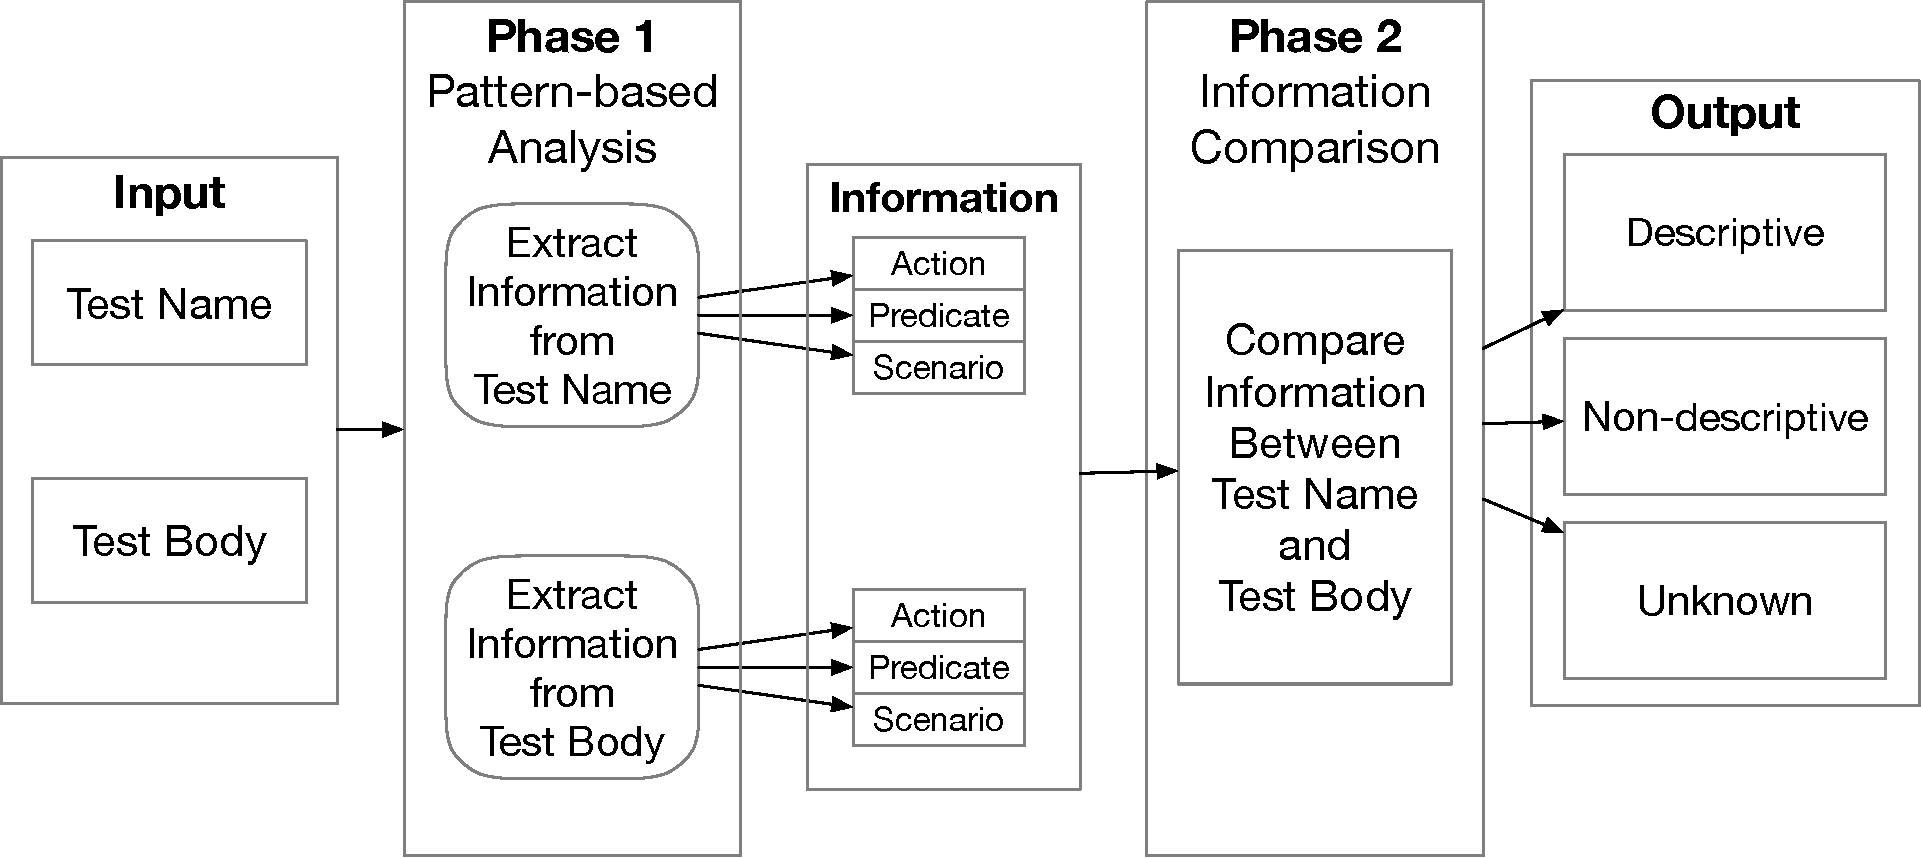
\includegraphics[scale=0.25]{figures/overview_of_approach.pdf}
  \caption{Overview of the pattern-based approach.}
  \label{fig:approach}
\end{figure*}

\item[Regex Match]

This name pattern is a collection of \num{70} regular expression-based sub-patterns.
%
For example, three of the most representative sub-patterns are shown in \cref{fig:regex-match}.
%
The first two sub-patterns show a special condition that need to perform the predicate under the defined scenario or execute the action after the scenario is performed.
%
The last sub-pattern is to execute the predicate while the right scenario is successfully performed, and a pattern match in practice is shown in \cref{PatternExample_detectedPoorName_code}.

\end{description}


\subsection{A Pattern-based Approach to Detect Non-descriptive Test Names}

\label{sec:approach}

\Cref{fig:approach} presents a high-level overview of our pattern-based approach for detecting non-descriptive test names.
%
As the figure shows, the approach takes as input a unit test comprised of its name and body.
%
It then assesses the descriptiveness of the test's name using two phases.
%
The first phase, \emph{pattern-based analysis}, uses the test patterns described in \cref{sec:test_patterns} to extract descriptive information from both the test name and the test body.
%
The second phase, \emph{information comparison}, compares the descriptive information extracted from the name and body against each other.
%
This information comparison process allows for not only detecting non-descriptive test names (i.e., mismatches between the information), but also in some cases indicating to developers how the name could be improved.
%
The remainder of this section describes the two steps of the approach in more detail.

\subsubsection{Phase 1: Pattern-based Analysis}

\begin{figure}[t]
    \centering
    \begin{subfigure}{0.9\textwidth}
        \includecode[java]{figures/approach-example.java}
        \caption{Example test that is matched by more than one name pattern and more than one body pattern.}
        \label{fig:approach-0}
    \end{subfigure}
    \\[1ex]
        \begin{subfigure}[b]{\columnwidth}
            \centering
            \begin{tabular}{rcc}
            \toprule
                      & Single Entity  & Verb Phrase With Prepended Test \\
            \midrule
            action    & GetSSLProtocol & Get \\
            predicate & ---            & --- \\
            scenario  & ---            & SSL \\
            \bottomrule
            \end{tabular}
            \caption{Comparison of information extracted by both matching name patterns for the test shown in \cref{fig:approach-0}.}
            \label{fig:approach-1}
        \end{subfigure}
    \\[1ex]
    \begin{subfigure}[b]{\columnwidth}
        \centering
        \begin{tabular}{rcc}
        \toprule
                  & Normal (Restricted) & Normal (Generalized) \\
        \midrule
        action    & getSSLProtocol    & getSSLProtocol \\
        predicate & assertNotNull     & assertNotNull \\
        scenario  & protocol          & --- \\
        \bottomrule
        \end{tabular}
        \caption{Comparison of information extracted by both matching body patterns for the test shown in \cref{fig:approach-0}.}
        \label{fig:approach-2}
    \end{subfigure}    
    \caption{Example to illustrate the ordering patterns is necessary.}
    \label{fig:approach-example}
\end{figure}

The first phase of the approach is relatively straightforward as it consists mainly of applying the patterns described in \cref{sec:name-patterns,sec:body-patterns} to the provided test name and body.
%
If a pattern matches against a name or body, the values it extracts as the action, predicate, and scenario are passed as input to the second stage.
%
If none of the name patterns match or none of the body patterns match, empty values are passed instead.


The main complexity in this phase arises from the fact that more than one pattern may match a name or body.
% 
For example, \cref{fig:approach-0} shows a unit test that can be matched by more than one pattern.
%
More specifically, the test's body can be matched by both the restricted and generalized versions of the \enquote{Normal} pattern and the test's name can be matched by both the \enquote{Single Entity} and \enquote{Verb Phrase With Prepended Test} patterns.


While more than one pattern may match the same name or body, there is often one pattern that is preferred either because it is more accurate at extracting information or it can extract more information.
%
For example, the difference in information extracted by matching patterns can be seen in \cref{fig:approach-1,fig:approach-2}.
%
Each of these figures, the rows show the values extracted as the action, predicate, and scenario for the patterns shown in the corresponding columns.
%
A dash (---) indicates an empty value that occurs when a pattern did not extract a value for the corresponding type of information.
%
\Cref{fig:approach-1} is an example of when one pattern may be more accurate at extracting information.
%
In this case, the \enquote{Single Entity} pattern correctly extracts \enquote{GetSSLProtocol} as the action and does not extract a value for the predicate or scenario while the \enquote{Verb Phrase With Prepended Test} pattern incorrectly identifies the action and scenario.
%
\Cref{fig:approach-2} is an example of when one pattern may extract more information.
%
In this case, both the \enquote{Normal (Restricted)} and \enquote{Normal (Generalized)} patterns correctly identify the action as \enquote{getSslProtocol} and the predicate as \enquote{assertNotNull} but only the \enquote{Normal (Restricted)} pattern identifies the scenario as \enquote{protocol}.
%
Because of this difference in performance, it is important to order the patterns to produce the best results.


The ordering of both name and body patterns in our approach is based on our understanding of the patterns, the intuition that more specific patterns should be tried before more general patterns, and the results of applying them to the applications shown in \cref{tab:test-corpus} as a pilot study.
%
In this pilot study, we tested ten different arrangements of the patterns and selected the one that produced the most accurate ordering.
%
More details about this evaluation process can be find in \cref{sec:evaluation:feasibility,sec:evaluation:accuracy}.
%
The resulting orders for the name patterns and body patterns are shown in \cref{tab:name-patterns,tab:rq1-body}, respectively.



\subsubsection{Phase 2: Information Comparison}


The goal of the information comparison phase is to detect non-descriptive test names.
%
Our approach fulfills this goal by comparing the information extracted from the test name and body.
%
The result of this comparison is that a test name is either:
\begin{enumerate*}[itemjoin*={{, or }}]
    \item Descriptive
    \item Non-descriptive
    \item Unknown
\end{enumerate*}.


More specifically, each piece of information extracted from a test's name is compared with its corresponding piece of information extracted from the test's body (i.e., action\textsubscript{name} with action\textsubscript{body}, predicate\textsubscript{name} with predicate\textsubscript{body}, and scenario\textsubscript{name} with scenario\textsubscript{body}).
% 
If the action, predicate, and scenario extracted from the name are all empty and\slash or the action, predicate, and scenario extracted from the body are all empty, the name is characterized as Unknown.
%
In this case, it is impossible to determine the quality of the name because an insufficient amount of information was extracted from the name or body.


\begin{figure}[t]
    \centering
    \begin{subfigure}{0.9\textwidth}
    \centering
        \includecode[java]{figures/approach/detected4.java}
        \caption{Example test with a descriptive name.}
        \label{PatternExample_detected4_code}
    \end{subfigure}
    \\[0.5ex]
    \begin{subfigure}{0.9\textwidth}
    \centering
        \begin{tabular}{rcc}
        \toprule
                  & Name    & Body    \\
        \midrule
        action    & GetGraphNode  & getGraphNode()     \\
        predicate & ---           & assertEquals()     \\
        scenario  & ---           & ---                \\
        \bottomrule
        \end{tabular}
        \caption{Extracted information for the test shown in \cref{PatternExample_detected4_code}.}
        \label{PatternExample_detected4}
    \end{subfigure}
    \caption{Example of a descriptive test name.}
    \label{fig:descriptive-examples}
\end{figure}


\begin{figure}[t]
    \centering
    \begin{subfigure}{0.8\textwidth}
    \centering
        \includecode[java]{figures/approach/detected1.java}
        \caption{Example test with a non-descriptive name.}
        \label{PatternExample_detectedPoorName_code}
    \end{subfigure}
    \\[0.5ex]
    \begin{subfigure}{0.9\textwidth}
    \centering
        \begin{tabular}{rcc}
        \toprule
                  & Name           & Body      \\
        \midrule
        action    & ---            & extract() \\
        predicate & ThrowException & ---       \\
        scenario  & TokenIsAbsent  & response  \\
        \bottomrule
        \end{tabular}
        \caption{Extracted information for the test shown in \cref{PatternExample_detectedPoorName_code}.}
        \label{PatternExample_detectedPoorName}
    \end{subfigure}
    \caption{Examples of a non-descriptive test name.}
    \label{fig:non-descriptive-examples}
\end{figure}


If there is sufficient information to compare, the approach checks each existing piece of information from the name against the corresponding information from the body.
%
If all of the existing pieces of information match, then the name is considered \emph{descriptive}.
%
\Cref{fig:descriptive-examples} shows an example of a test name that is classified as descriptive.
%
The top of the figure shows the test under consideration and the bottom presents a table showing the information extracted by the first phase of the approach.
%
The rows of the table show the values extracted by the pattern type shown in the corresponding column (i.e., the name pattern identified \enquote{GetGraphNode} as the action and the body pattern identified \enquote{getGraphNode()} as the action).
%
In this example, the name is considered descriptive because all of the non-empty information types match their counterpart (i.e., \enquote{GetGraphNode} matches \enquote{getGraphNode()}).


If, when comparing the name information against the body information, at least one of the existing pieces of information does not match, then the name is considered \emph{non-descriptive}.
%
It means that a subset of the following conditions happens for that name:
\begin{enumerate*}[itemjoin*={{, or }}]
    \item action\textsubscript{name} does not match action\textsubscript{body}
    \item predicate\textsubscript{name} does not match predicate\textsubscript{body}
    \item scenario\textsubscript{name} does not match scenario\textsubscript{body}
\end{enumerate*}.
%
\Cref{fig:non-descriptive-examples} shows an example of name that is classified as non-descriptive.
%
Again, the top of the figure shows the test under consideration and the bottom presents a table showing the information extracted by the first phase of the approach.
%
In this example, the name is considered non-descriptive because none of the non-empty information types match their counterpart (i.e., \enquote{TokenIsAbsent} fails to match \enquote{response}).


If the outcome is either descriptive or non-descriptive, the approach can sometimes provide additional information to developers to help them improve the test name.
%
For both descriptive and non-descriptive names, if a value provided by the name pattern is empty but the corresponding information provided by the body is not empty, the name can likely be improved by the addition of the body information.
%
For example, \cref{PatternExample_detected4} shows a test name that is descriptive but can also be improved.
%
In this example, the name accurately reflects that the action of the test is \enquote{GetGraphNode} but it is missing information about the predicate that can be found in the body.
%
Adding information that the predicate is \enquote{assertEquals} to the name would improve its descriptiveness.


For only non-descriptive names, the approach can suggest modification in two cases.
%
First, if a value provided by the name pattern exists but the corresponding value provided by the body pattern does not exist, the approach suggests that the name information from the name be removed as it is not supported by the body.
%
Second, if the corresponding values provided by the name and body patterns both exist but do not match, the approach can suggest that the information from the name be replaced by the information from the body.
%
For example, \cref{PatternExample_detectedPoorName} shows a non-descriptive test name, which the approach can provide the following suggestions for improvement:
%
First, the predicate part of the name, \enquote{ThrowException}, should be removed and second, the scenario identified by the name, \enquote{TokenIsAbsent}, should also be replaced with the scenario from the body, \enquote{response}.
%
Note that, because the action from the name is empty, the action identified by the body, \enquote{extract}, should be added to the name, as described above.


The challenging part of this phase is determining whether the corresponding pieces of information match.
%
Because the information extracted from the name is text while the information extracted from the body are code elements (i.e., \texttt{methods}, \texttt{objects}, etc.) they can not be directly compared.
%
To address the challenge, the approach automatically converts the \emph{name} of any \texttt{method}, \texttt{object}, \texttt{new instance}, or \texttt{assertion method} to a string.
%
For example, the \enquote{Normal (Restricted)} body patterns can extract the name of the \texttt{assertion method} in \cref{fig:approach-0}, and it is converted to a string that is shown as \enquote{assertNotNull} in \cref{fig:approach-2}.
%
Once both the information from the name and the information from the body have been converted to strings, they are also converted to lower case.
%
The two string are equal, or if one is strictly contained in the other, they are considered to match.
%
Otherwise, they are unmatched.

\subsection{Empirical Evaluation}
\label{sec:evaluation}


The overall goal of the evaluation is to determine if our approach can classify descriptive and non-descriptive test names. 
%
However, because the approach's success for this task depends on the underlying patterns, we also evaluate several aspects of their performance.
%
More specifically, we considered the following three research questions:
\begin{description}[font=\normalfont\emph]
\item[RQ1---Feasibility.] How many test names and bodies are matched by the patterns used by the approach?
\item[RQ2---Accuracy.] How accurate are the patterns at extracting the action, scenario, and predicate from test names and bodies?
\item[RQ3---Effectiveness.] Can our pattern-based approach correctly classify descriptive and non-descriptive test names?
\end{description}


To investigate these questions, we implemented our approach as an IntelliJ IDEA Plugin \cite{IntelliJPlugin}.
%
We chose to use IntelliJ IDEA because it is a full-featured IDE that can import projects which use a wide variety of build systems (e.g., Maven and Gradle).
%
This gives us more flexibility in choosing applications when building our set of experimental subjects.
%
It also has support for automatically identifying test suites, which are the input to the approach.
%
Finally, it has a robust parsing API that we can use to implement the body patterns.


To generate the experimental data for investigating our research questions, we instrumented the plugin to record the information necessary for answering each research question.
%
We then manually ran the plugin on each of the experimental subjects.
%
For each run, the plugin automatically imports the project that is going to be evaluated.
%
After the importing finishes, the plugin will attempt to match every test pattern on each unit test that is contained in that imported project.
%
Finally, the plugin outputs a report for all unit tests that are evaluated in the process.
%
In total, we collected all information comparison reports for each of the ten Java projects we used in the evaluation.
%
The machine we used for all experiments was a MacBook Pro (\SI{2.7}{\giga\hertz} Intel i5 processor; 16 GB RAM) running macOS High Sierra and Java version 9.0.1.
%
Adding up the time for executing the plugin on each project, the total amount of time is roughly five hours for \num{34352} tests.
%
Even though the implementation is unoptimized, the execution time is such that it is feasible to include the approach as part of an off-line build process (e.g., overnight).


The remainder of this section describes our experimental subjects and research questions in more detail.


\subsubsection{Experimental Subjects}
\label{sec:evaluation:subjects}

\begin{table*}
\centering
\begin{tabular}{
  l
  l
  S[table-format=5]
}
 \toprule 
 \multicolumn{1}{c}{\textbf{Project}} & \multicolumn{1}{c}{\textbf{Commit}} & \multicolumn{1}{c}{\textbf{\# Tests}} \\
 \midrule
 Xodus      & 8d82ef7 & 940   \\
 mytcuml    & 0786c55 & 21532 \\
 wheels     & 15696da & 811   \\
 EventBus   & 2e7c046 & 124   \\
 Picasso    & 5c05678 & 336   \\
 Jenkins    & 6c1d61a & 2245  \\
 ScribeJava & fce41f9 & 109   \\
 mockito    & 2204944 & 2112  \\
 Guice      & 6f1c6cc & 1322  \\
 fastjson   & 4c7935c & 4821  \\
 \midrule
 \multicolumn{2}{r}{Total} & 34352 \\
 \bottomrule
\end{tabular}
\caption{Experimental Subjects.}
\label{tab:subjects-pattern}
\end{table*}


As the subjects for the evaluation, we selected a set of \num{34352} unit tests comprised of the test suites from the \num{10} Java projects shown in \cref{tab:subjects-pattern}.
%
In the table, the first column, \emph{Project}, shows the name of each project; the second column, \emph{Commit}, shows commit hash of the version of the project that was evaluated; and the last column, \emph{\#~Tests}, shows the number of unit tests contained in each project's test suite.


We chose these projects for several reasons.
%
First, they are distinct from the applications and test suites we used to develop the patterns (see \cref{sec:test_patterns}).
%
Clearly, the patterns should perform well on the tests that they were derived from.
%
Having separate test suites allows for a more representative evaluation of the first two research questions.
%
Second, the applications they test are diverse since they cover a wide variety of application domains.
%
For example, \enquote{Xodus} is a transactional database, \enquote{mytcuml} is a UML tool, \enquote{wheels} is a testing framework, and \enquote{EventBus} is a publish\slash subscribe pattern-based library that can simplify Android and Java code.
%
In addition, they were written by different developers and at different times.
%
This means that the test suites are not limited to a particular set of authors or patterns and are more likely to be representative than any test from a single project or style.
%
Finally, in aggregate, they have a sufficient number of tests to allow for a thorough evaluation of the approach.


\subsubsection{RQ1: Feasibility}
\label{sec:evaluation:feasibility}

\begin{table*}[t]
\centering
\begin{tabular}{
  l
  S[table-format=5]
  S[table-format=3.2]
}
 \toprule 
 \multicolumn{1}{c}{\textbf{Name Pattern}} & \multicolumn{1}{c}{\textbf{\# Matches}} & \multicolumn{1}{c}{\textbf{(\%)}} \\
 \midrule
 Verb With Multiple Nouns Phrase           & 0                                       & 0.00  \\
 Divided Duel Verb Phrase                  & 0                                       & 0.00  \\
 Is And Past Participle Phrase             & 0                                       & 0.00  \\
 Try Catch                                 & 204                                     & 0.59  \\
 Duel Verb Phrase                          & 331                                     & 0.96  \\
 Noun Phrase                               & 1555                                    & 4.53  \\
 Single Entity                             & 4794                                    & 13.96 \\
 Verb Phrase Without Prepended Test        & 2578                                    & 7.50  \\
 Verb Phrase With Prepended Test           & 9007                                    & 26.22 \\
 Regex Match                               & 15883                                   & 46.24 \\
 \midrule
 Overall                                   & 34352                                   & 100.00 \\
 \bottomrule
\end{tabular}
\caption{Match Rate for Name Patterns.}
\label{tab:rq1-name}
\end{table*}

\begin{table*}[t]
\centering
\begin{tabular}{
  l
  S[table-format=5]
  S[table-format=3.2]
}
 \toprule 
 \multicolumn{1}{c}{\textbf{Body Pattern}} & \multicolumn{1}{c}{\textbf{\# Matches}} & \multicolumn{1}{c}{\textbf{(\%)}} \\
 \midrule
 If Else                                   & 17                                      & 0.05   \\
 Loop                                      & 533                                     & 1.55   \\
 All Assertion                             & 1801                                    & 5.24   \\
 No Assertion                              & 3602                                    & 10.49  \\
 Try Catch                                 & 5075                                    & 14.77  \\
 Normal (Restricted)                       & 1634                                    & 4.76   \\
 Normal (Generalized)                      & 13840                                   & 40.29  \\
 \midrule
 Overall                                   & 26502                                   & 77.15  \\
 \bottomrule
\end{tabular}
\caption{Match Rates for Body Patterns.}
\label{tab:rq1-body}
\end{table*}


The purpose of the first research question is to evaluate the feasibility of our pattern-based approach.
%
The primary way in which we judge feasibility is to determine the percentage of test names and bodies that are matched by one of the patterns used by the approach.
%
In some sense, this is the \enquote{coverage} of the patterns.
%
If the coverage of the patterns is low, the usefulness of the approach will also be low as the approach will only be able to provide feedback for a small number of tests.
%
Conversely, if the coverage of the patterns is high, the approach is potentially more useful as it can provide feedback for more tests.
%
However, there is a potential trade-off between the coverage of the patterns and their accuracy (see \cref{sec:evaluation:accuracy}) in that increasing coverage may result in lower accuracy.
%
As such, the sweet-spot for the approach is achieving enough coverage to enable providing feedback for most tests, but not compromising the accuracy of the extracted information.


\Cref{tab:rq1-name,tab:rq1-body} show the experimental data for this research question.
% 
In each table, the first column, \emph{Name\slash Body Pattern}, shows the name of each pattern; the final two columns, \emph{\# Matches} and \emph{\%}, show the number of times the pattern matched against a test both as a count and a percentage, respectively; and the final row shows an overall summary of the results.
%
For example, the fourth row of \cref{tab:rq1-name} shows that \enquote{Try Catch} matched \num{204} test names (i.e., \SI{\approx 0.6}{\percent} of the \num{34352} considered test names).
%
Similarly, the first row of \cref{tab:rq1-body} shows that \enquote{If Else} matched \num{17} of the \num{34352} considered test bodies (i.e., \SI{\approx 0.05}{\percent} of the \num{34352} considered test bodies).
% 
Note that, to simplify the tables and the discussion, most variations of a pattern are grouped into a single row.  For example, in \cref{tab:rq1-body}, \enquote{All Assertion} includes both the \enquote{Single} and the \enquote{Multiple} versions presented in \cref{tab:body-patterns}.


As the final row in each table shows, the overall match rate for both name and body patterns is high.
%
In aggregate, the name patterns matched \num{34352} test names (i.e., \SI{100}{\percent}), and the body patterns matched \num{26502} test bodies (i.e., \SI{\approx 77}{\percent}).
%
While there are a few patterns that had low or zero match rates (e.g., \enquote{Divided Duel Verb Phrase}), the cost of keeping such patterns is low as their execution times are low and they may be more prevalent in other project types.
%
The data also demonstrate that the ordering of the patterns is effective.
%
More general patterns (i.e., ones have shown lower in the tables) have higher match rates than more specific patterns (ones shown higher in the tables).
%
Overall, we believe that these results suggest that the approach is feasible.
%
The coverage of the patterns is high enough to enable the approach to provide feedback for a majority of tests.


\subsubsection{RQ2: Accuracy}
\label{sec:evaluation:accuracy}


\begin{table*}[t]
\begin{adjustbox}{max width=\textwidth}
\begin{tabular}{
l
S[table-format=3.1]
S[table-format=3.1]
S[table-format=3.1]
S[table-format=3.1]
S[table-format=3.1]
S[table-format=3.1]
}
 \toprule 

 &  \multicolumn{2}{c}{\textbf{Action (\%)}}  &  \multicolumn{2}{c}{\textbf{Predicate (\%)}}  & \multicolumn{2}{c}{\textbf{Scenario (\%)}} \\
 
 \cmidrule(lr){2-3} \cmidrule(lr){4-5} \cmidrule(lr){6-7}
 
\multicolumn{1}{c}{\textbf{Name Pattern}} & \multicolumn{1}{c}{\textbf{TP}} & \multicolumn{1}{c}{\textbf{FP}} & \multicolumn{1}{c}{\textbf{TP}} & \multicolumn{1}{c}{\textbf{FP}} & \multicolumn{1}{c}{\textbf{TP}} & \multicolumn{1}{c}{\textbf{FP}} \\
 \midrule
  Verb With Multiple Nouns Phrase    & {---} & {---} & {---} & {---} & {---} & {---} \\
  Divided Duel Verb Phrase           & {---} & {---} & {---} & {---} & {---} & {---} \\
  Is And Past Participle Phrase      & {---} & {---} & {---} & {---} & {---} & {---} \\
  Try Catch                          & 89  & 11 & 96  & 4  & 89  & 11                \\
  Duel Verb Phrase                   & 96  & 4  & 88  & 12 & 84  & 16                \\
  Noun Phrase                        & 100 & 0  & 100 & 0  & 100 & 0                 \\
  Single Entity                      & 97  & 3  & 97  & 3  & 89  & 11                \\
  Verb Phrase With Prepended Test    & 87  & 13 & 74  & 26 & 95  & 5                 \\
  Verb Phrase Without Prepended Test & 100 & 0  & 75  & 25 & 75  & 25                \\
  Regex Match                        & 84  & 16 & 84  & 16 & 72  & 28                \\
  \midrule
  Overall                            & 92  & 8  & 87  & 13 & 89  & 11                \\
 \bottomrule
\end{tabular}
\end{adjustbox}
\caption{Accuracy Results for Each Name Pattern.}
\label{tab:rq2_name}
\end{table*}

\begin{table*}[t]
\centering
\begin{tabular}{
  l
  S[table-format=3.1]
  S[table-format=3.1]
  S[table-format=3.1]
  S[table-format=3.1]
  S[table-format=3.1]
  S[table-format=3.1]
}
\toprule 
 &  \multicolumn{2}{c}{\textbf{Action (\%)}}  &  \multicolumn{2}{c}{\textbf{Predicate (\%)}}  & \multicolumn{2}{c}{\textbf{Scenario (\%)}} \\
 
 \cmidrule(lr){2-3} \cmidrule(lr){4-5} \cmidrule(lr){6-7}
 
\multicolumn{1}{c}{\textbf{Body Pattern}} & \multicolumn{1}{c}{\textbf{TP}} & \multicolumn{1}{c}{\textbf{FP}} & \multicolumn{1}{c}{\textbf{TP}} & \multicolumn{1}{c}{\textbf{FP}} & \multicolumn{1}{c}{\textbf{TP}} & \multicolumn{1}{c}{\textbf{FP}} \\
 \midrule
  If Else              & 91  & 9  & 36  & 64 & 100 & 0 \\
  Loop                 & 89  & 11 & 86  & 14 & 94  & 6 \\
  All Assertion        & 100 & 0  & 89  & 11  & 100 & 0 \\
  No Assertion         & 96  & 4  & 74  & 26 & 100 & 0 \\
  Try Catch            & 100 & 0  & 94  & 6  & 91  & 9 \\
  Normal (Restricted)  & 100 & 0  & 100 & 0  & 100 & 0 \\
  Normal (Generalized) & 82  & 18 & 100 & 0  & 96  & 4 \\
  \midrule
  Overall              & 94  & 6  & 88  & 12 & 97  & 3 \\
 \bottomrule
\end{tabular}
\caption{Accuracy Results for Each Body Pattern.}
\label{tab:rq2_body}
\end{table*}


The goal of the second research question is to investigate whether the patterns can accurately extract information from test names and bodies.
%
Because assessing the accuracy of the extracted information must be done manually, it is infeasible to consider all \num{26502} tests that were matched by a pattern.
%
Therefore, we chose a subset of information extracted from matched tests to classify.
%
For each name pattern and each body pattern, we randomly selected up to \num{5} tests matched by that pattern from each project.
%
If no test was matched by that pattern in a project, we skipped the project and moved on to the next one.
%
In total, \num{242} tests were selected for the name patterns and \num{266} tests were selected for the body patterns.


For each test in the selected subset, each author manually examined the information extracted by the matching name and body patterns independently.
%
If the extracted information matched the human's judgment it was considered a true positive (TP) and if the extracted information did not match the human's judgment it was considered a false positive (FP).
%
Disagreements among the raters were discussed until a resolution was reached.
%
In total, \num{1524} comparisons were made by each rater (i.e., (\num{242} tests for name patterns + \num{266} tests for body patterns) * \num{3} comparisons, the action, predicate, and scenario for each test).


\Cref{tab:rq2_name,tab:rq2_body} show the experimental data for this research question.
%
\Cref{tab:rq2_name} shows the accuracy of the name patterns and \cref{tab:rq2_body} shows the accuracy of the body patterns.
%
In each table, the first column is the name of each pattern, and the following three pairs of columns show the TP and FP rates for the information extracted as the action, predicate, and scenario by each pattern.
%
The final row shows the overall rates for all patterns.
%
For example, the fourth row of \cref{tab:rq2_name} shows the accuracy results for the \enquote{Try Catch} name pattern: the TP rate for the action is \SI{89}{\percent}, the TP rate for the predicate is \SI{96}{\percent}, and the TP rate for the scenario is \SI{89}{\percent}.
%
Note that in \cref{tab:rq2_name} a dash (---) indicates the cases where a manual assessment was impossible because the patterns did not match any tests.


The data shown in \cref{tab:rq2_name} and \cref{tab:rq2_body}, indicates that the overall accuracy of both the name patterns and body patterns is high.
%
For name patterns, the overall true positive rates range from \SI{87}{\percent} for the scenario to \SI{92}{\percent} for the action and for the body patterns the overall true positive rates range from \SI{88}{\percent} for the predicate to \SI{97}{\percent} for the scenario.
%
Even in the worst cases (e.g., identifying the scenario with the Regex Match name pattern), the true positive rate is above \SI{70}{\percent}.
%
As such, we believe that both types of patterns are effective at accurately identifying the action, predicate, and scenario from tests.


\subsubsection{RQ3: Effectiveness}

\begin{table*}[t]
\centering
\begin{tabular}
{
  l
  S[table-format=3]
  S[table-format=2.1]
}
\toprule 
\multicolumn{1}{c}{\textbf{Classification}} & \multicolumn{1}{c}{\textbf{Count}} & \multicolumn{1}{c}{\textbf{(\%)}}\\
\midrule
TP  & 251 & 94.7 \\
FP  & 14  & 5.3  \\
\bottomrule
\end{tabular}
\caption{Effectiveness of the approach.}
\label{tab:rq3}
\end{table*}


The goal of the third research question is to determine if the pattern-based approach can correctly classify descriptive and non-descriptive test names.
%
Like for RQ2, assessing the output of the approach is a manual process that can not be applied to every output.
%
Therefore, we again selected a representative subset to consider.
%
In this case, because we are interested in the performance across all tests, we chose to consider a total of  \num{265} tests (i.e., \SI{1}{\percent} of the \num{26502} tests matched by both a name and body pattern).
%
The \num{265} tests were selected from among each project proportionally to the number of tests in the project's test suite (e.g., \num{166} tests were taken from \enquote{mytcuml}, \num{37} test were taken from \enquote{fastjson}, etc.).


For each test in the selected subset, each author again manually examined the output of the approach independently.
%
If the output of the approach matched the human's judgment it was considered a true positive (TP) and if the output did not match the human's judgment it was considered a false positive (FP).
%
Disagreements among the raters were discussed until a resolution was reached.
%
The results of the classification are shown in \cref{tab:rq3}.


In \cref{tab:rq3}, the first column shows the classification of reports (i.e., either a true-positive~(TP) or a false-positive~(FP)), and the second and third columns show the number of true and false positives as a raw count and as a ratio out of the total number of reports (i.e., \num{265}).
%
For example, the first number in the first row shows there are \num{251} reports (\SI{\approx 95}{\percent}) that correctly classify a test name as either descriptive or non-descriptive.
%
Because the true positive rate is high, we can conclude that the pattern-based approach is effective at classifying names as either descriptive or non-descriptive.

\subsection{Conclusions}

Taking every test pattern into consideration, our selected test patterns can extract sufficient information from any unit test with matched name\slash body patterns.
%
With the help of the output generated by our approach, developers can easily find non-descriptive test names from a given test corpus and improve those non-descriptive names by referring to the descriptive information.
%
Furthermore, we also implemented our approach as an IntelliJ IDE plugin.
%
In the empirical evaluation, the experimental results produced by our implemented approach are encouraging, which show our approach not only can accurately extract descriptive information from unit tests but also can correctly classify descriptive and non-descriptive test names.


\end{document}

\subsection{An Empirical Study of Unit Test Naming Rationales}
\label{sec:emp-study}

As the first component towards generating descriptive test names, I conducted an empirical study to understand existing test naming rationales.
%
My intuition is that developers often name unit tests based on what aspects of the test makes the test unique among its siblings.
%
To validate this assumption, I conducted an empirical study of \num{440} existing tests.
%
First, I examined each test in order to identify what makes it unique from its siblings.
%
Then I examined the test’s name and judged whether the name is based either entirely or in part on the unique aspect of the test.


\subsubsection{Study Methodology}

As the first part of this study, I randomly selected a set of \num{440} tests from \num{11} open-source projects from Github.
%
Moreover, I used an open, axial, and selective coding process to qualitatively analyze the tests.
%
Finally, I discussed the results of the coding process and the data to answer two research questions about whether unit tests are named, either wholly or in part, after what makes a given test unique among its siblings.


\paragraph{Experimental Subjects}

To gather the tests we examined in our study, we started with the \num{11} Java projects shown in~\cref{tab:subjectsForStudy}.
%
In the table, the first column, \emph{Name}, shows the name of the project; the second column, \emph{Version}, shows the version of the project (either as a Git hash or version number); the fourth column, \emph{LoC}, shows the number of non-comment, non-blank lines of code as computed by SLOC count~\cite{nguyen2007sloc}; and the final column, \emph{\# Tests}, shows the number of unit tests in the project. In total, these \num{11} projects contain \num{25459} unit tests.


The first ten projects were randomly selected from the top \num{50} Java projects hosted on Github~\cite{top50projects}.
%
Because these projects encompass a variety of domains (e.g., JavaPoet is a library for generating Java programmatically and ExoPlayer is a media player for Android) and have many contributors (e.g., Moshi’s test suite contains contributions from \num{8} different people), their tests are more likely to be representative of tests in general which helps mitigate a potential threat to validity.
%
In addition, we also included Barbecue, a commonly used subject in the testing literature (e.g.,~\cite{zhang2015automatically, zhang2016towards,wu2020pattern}).
%
Because Barbecue is significantly smaller than the other subjects, it served as a useful starting point for the study.


Because our investigation is manual, it is necessary to reduce the \num{25459} unit tests to a more manageable number.
%
Because the projects vary widely in their numbers of tests (e.g., Guava contains \num{13962} tests while socket.io-client contains \num{85} tests), we decided to select a fixed number of tests from each project rather than choosing in proportion to test suite size.
%
This also helps control for threats associated with an unbalanced sample.
%
We found that it took about \num{5} minutes to understand and encode a single test.
%
Therefore, referencing from similar studies~\cite{wu2020pattern,zhang2016towards}, we selected \num{40} tests from each project, giving us a total of \num{440} tests; an amount which could be analyzed in around \num{37} hours (i.e., approximately a week’s worth of effort).


When performing the selection of tests, we also had an additional requirement which was to only select tests without poor names.
%
Prior work has demonstrated that tests often have poor names (e.g., test1, test2, etc.)~\cite{zhang2016towards}.
%
Because we are not interested in generating poor names nor understanding how poor names are chosen (although this may be an interesting area of future work), it makes sense to eliminate tests with poor names from consideration.
%
Therefore, if a randomly selected test had a name that the authors judged was poor it was replaced with another randomly selected test.
%
We considered a name to be poor if, with the exception of a leading \enquote{test}, the name contains only numbers (e.g., test12) or numbers and symbols (e.g., test\_2\_3).
%
We also made sure not to select any of the \num{179} tests with empty bodies contained in these applications.
% TODO [Fixed]: fix URL 
The final set of \num{440} tests is available online~\cite{emp-data}.

\begin{table}[t]
\centering
\caption{Experimental Subjects.\strut}
\begin{tabular}
{
  l
  l
  S[table-format=5.1]
  S[table-format=5.1]
}
\toprule
\multicolumn{1}{c}{\textbf{Project}} &
\multicolumn{1}{c}{\textbf{Version}} & 
\multicolumn{1}{c}{\textbf{LoC}} &
\multicolumn{1}{c}{\textbf{\# Tests}}
\\
\midrule
 Guice             & 9b371d3 &  183049  & 1280   \\
 Moshi             & dbed99d  &  22168  & 716   \\
 Picasso           & a087d26  &  11006  & 229  \\
 Fastjson          & e05f1f9  &  195511  & 4950   \\
 Guava             & 368c337  &  400801  & 13962  \\
 Mockito           & 22c82dc   &  59839 & 2145   \\
 Socket.io-client  & 661f1e7  &  9478  & 85  \\
 Scribejava        & ea42bc9  &  15184  & 110   \\
 ExoPlayer         & 79da521  &  172148  & 1510   \\
 Javapoet          & e9460b8  &  10755  & 302   \\
 Barbecue          & 44a8632  &  10760  & 170   \\
\bottomrule
\end{tabular}
\label{tab:subjectsForStudy}
\end{table}

\paragraph{Code Creations}

The goal of the first part of our study is to identify what makes tests unique.
%
Note that in this work we are assuming that each test has some aspect that makes it unique.
%
While we have observed cases where more than one test has the same body (i.e., duplicate tests with different names), this situation is rare, did not occur among our set of tests, and is likely indicative of a bug as there is no obvious benefit to executing the same test twice.

Identifying what makes a test unique involves comprehending not only the test under consideration but also the test's siblings (i.e., tests that influence or restrict the name of a test).
%
In this study we consider tests declared in the same class as siblings. 
%
We chose this granularity for several reasons.
%
First, the Java programming language forbids methods with the same signature in the same class.
%
Because tests have no parameters, this means that each test (method) in a class must have a unique name.
%
Second, tests in the same class are likely to be related (e.g., they share the same class under test).
%
This means that the aspects that make them unique are more likely to be limited in scope and therefore more interesting with respect to how tests are named.

Because there is no pre-existing classification scheme for identifying what makes a test unique, we used open, axial, and selective coding to qualitatively analyze the tests~\cite{glaser1967discovery, strauss1998basics}.
%
First, each author examined each of the \num{440} considered tests and tagged the portions of the test body that they believe are the unique aspects of the test.
%
Each tag consisted of a word or short phrase that characterizes the type of uniqueness.
%
After each author tagged each test individually, the authors together examined the tagged tests in order to reach consensus on which portion of a test's body makes it unique and to discuss the open codes.
%
Then the authors used axial coding to establish relationships among the open codes and generated a final list of selective codes.

The set of selective codes is based partly on the Java language elements~\cite{Oracle-Classes} that can comprise a test (e.g., variable declarations, method calls, control flow structures, parameters and arguments, etc.).
%
However, we found that it was desirable to both refine these codes and to include other, more broad codes, in order to more precisely capture concepts that are specific to unit tests.
%
More specifically, we created four top-level codes that correspond to the high-level structure of the test (i.e., parts of test~\cite{zhang2016towards}) and multiple secondary codes that refer to test-specific elements (e.g., calls to methods of the class under test, expected or actual arguments to assertions, etc).
%
Because secondary codes refine top-level codes, they can only be applied if their corresponding top-level is applied first. 
%
Below, we discuss each top-level code and its associated secondary codes in detail.

\subparagraph{Action}

The Action code is a top-level code that is applied to a test when no sibling test shares the test's Action---the part of the test that is the primary interaction with the application under test.
%
The secondary codes for the Action code relate to:
\begin{enumerate*}
\item the elements of the action, specifically methods calls and arguments
\item whether the method calls and arguments are related to the class under test
\end{enumerate*}.

Because, in the context of testing, method calls to the class under test are more important than calls to methods declared by other classes and method calls in general are more important than method arguments, the secondary codes are prioritized as shown below; a lower ranked code can only be applied if no high-ranked code has been applied.
%
This ranking is based on our intuition as well as recent studies that use eye-tracking technology to understand the importance of code elements for different software engineering tasks (e.g., \cite{rodeghero2015empirical, rodeghero2015eye, begel2018eye}).

\begin{enumerate}
\item The CUT Method Call code is applied when 
\begin{enumerate*}[label=(\roman*)]
\item the test’s action contains a call to a method declared by the class under test (CUT) 
\item no other sibling test contains a call to the same method in its action, irrespective of the method arguments
\end{enumerate*}

\item The non-CUT (other) Method Call code is applied when 
\begin{enumerate*}[label=(\roman*)]
\item the test’s action contains a call to a method declared by a class that is not the class under test 
\item no other sibling test contains a call to the same method in its action, irrespective of the method arguments
\end{enumerate*}

\item The CUT call arguments code is applied when the test’s action contains a call to a method declared by the class under test (CUT) that has a unique set of method call arguments

\item The non-CUT (other) call arguments code is applied when the test’s action contains a call to a method declared by a class that is not the class under test that has a unique set of method call arguments.
\end{enumerate}

\subparagraph{Predicate}

The Predicate code is applied to a test when no sibling test shares the test’s predicate---the part of the test that checks the result of the performing the action.
%
The secondary codes for the Predicate code relate to: 
\begin{enumerate*}
\item the assertions used by the test and 
\item the arguments passed to the assertions
\end{enumerate*}.
%
Again, the secondary codes are prioritized based on their relative importance in the context of testing and a lower-ranked code can only be applied if a higher-ranked code has not already been used.
%
The Predicate code has noticeably more secondary codes than other top-level codes.
%
First, the definition of unit testing is to test a minimum component of a software, so the testing process is usually involved with checking the produced results.
%
Second, when checking the produced results, there are many different kinds of result-checking statements that can be used in a test, which will make the test unique.

\begin{enumerate}

\item The actual and expected parameters code is applied when 
\begin{enumerate*}[label=(\roman*)]
\item the test’s predicate contains a pair of actual and expected parameters that is extracted from an assertion call 
\item no other sibling test has the same pair of actual and expected parameters in its assertion calls
\end{enumerate*}

\item The actual parameter code is applied when 
\begin{enumerate*}[label=(\roman*)]
\item the test’s predicate contains an actual parameter that is extracted from an assertion call 
\item no other sibling test has the same actual parameter in its assertion calls
\end{enumerate*}

\item The expected parameter code is applied when 
\begin{enumerate*}[label=(\roman*)]
\item the test’s predicate contains an expected parameter that is extracted from an assertion call 
\item no other sibling test has the same expected parameter in its assertion calls
\end{enumerate*}

\item The assertion call code is applied when 
\begin{enumerate*}[label=(\roman*)]
\item the test’s predicate contains an assertion call that is extracted from the assertions of the test 
\item no other sibling test has the same assertion call and uses it as its predicate
\end{enumerate*}

\item The other result-checking call code is applied when 
\begin{enumerate*}[label=(\roman*)]
\item the test’s predicate contains other types of result-checking calls that serve the same functionality as JUnit assertions 
\item no other sibling test has the same set of result-checking calls and uses it as its predicate
\end{enumerate*}

\item The only assertion code is applied when the test’s predicate contains a call to an JUnit assertion method and no other sibling test calls any JUnit assertion method (i.e., the only test with JUnit assertion).

\end{enumerate}


\subparagraph{Scenario}

The Scenario code is applied to a test when no sibling test shares the test’s scenario---the part of the test that configures or sets up the environment under which the action will be performed.

The secondary codes for the Scenario code relate to:
\begin{enumerate*}[label=(\roman*)]
\item the elements of the scenario, specifically variable initialization and arguments in assertions
\item whether the variable initialization and arguments are related to the object under test
\item control flow variable and state-changing CUT call
\end{enumerate*}.

Because, in the context of testing, variable initialization to the object under test are more important than variable initialization to other objects and variable initialization in general are more important than variable initialization arguments and control flow variables.
%
And the state-changing CUT method call code is added in the list to meet the possible case of having a focal method call \cite{ghafari2015automatically}.
%
Therefore, the secondary codes are prioritized as shown below and a lower ranked code can only be applied if no high-ranked code has been applied.

\begin{enumerate}
    
    \item The OUT variable initialization code is applied when
    \begin{enumerate*}[label=(\roman*)]
        \item the test’s scenario contains a variable initialization that is used in a variable declaration for an object under test (OUT) 
        \item no other sibling test contains the same variable initialization for its variable declaration for OUT and uses it as its scenario, irrespective of the arguments used in the variable initialization. The OUT variable initialization will be the tagged text, and the rest of the secondary code of the Scenario code follows the same rule (i.e., code elements are converted to the tagged text)
    \end{enumerate*}.

    \item The non-OUT (other) variable initialization code is applied when
    \begin{enumerate*}[label=(\roman*)]
        \item the test’s scenario contains a variable initialization that is used in a variable declaration but not for any object under test 
        \item no other sibling test contains the same variable initialization for its variable declaration (i.e., not for OUT) and uses it as its scenario, irrespective of the arguments used in the variable initialization
    \end{enumerate*}.
    
    \item The non-OUT (other) variable initialization arguments code is applied when 
    \begin{enumerate*}[label=(\roman*)]
    	\item the test’s scenario is composed of a set of arguments that are used in the variable initialization of a variable declaration but not for any object under test
    	\item no other sibling test contains the same set of arguments that are used in variable initialization of a non-OUT variable declaration and uses it as its scenario
    \end{enumerate*}.
    
    \item The control flow variable code is applied when 
    \begin{enumerate*}[label=(\roman*)]
        \item the test’s scenario contains a variable that is used in the conditional statement of a control flow-based statement (i.e., loop, if-else, or other type of statement)
        \item no other sibling test contains the same variable that is used in the same type of control flow-based statement and uses it as its scenario
    \end{enumerate*}.
    
    \item The state-changing CUT method call code is applied when
    \begin{enumerate*}[label=(\roman*)]
        \item the test scenario is composed of a CUT method call that changes the state of the test~\cite{ghafari2015automatically}
        \item no other sibling test contains the same state-changing CUT method call in its scenario, irrespective of the method arguments
    \end{enumerate*}.

\end{enumerate}

\begin{figure}[t]
\centering
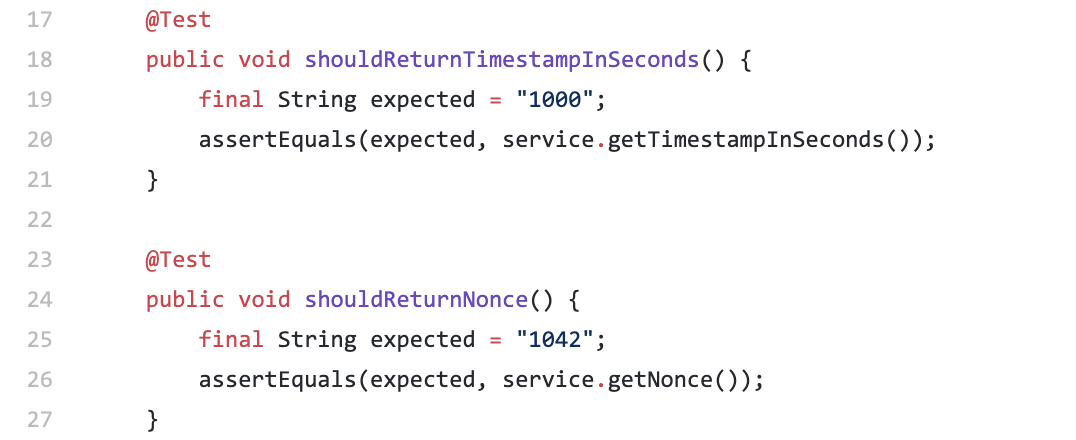
\includegraphics[scale=0.45]{figures/sp3-proposal.png}
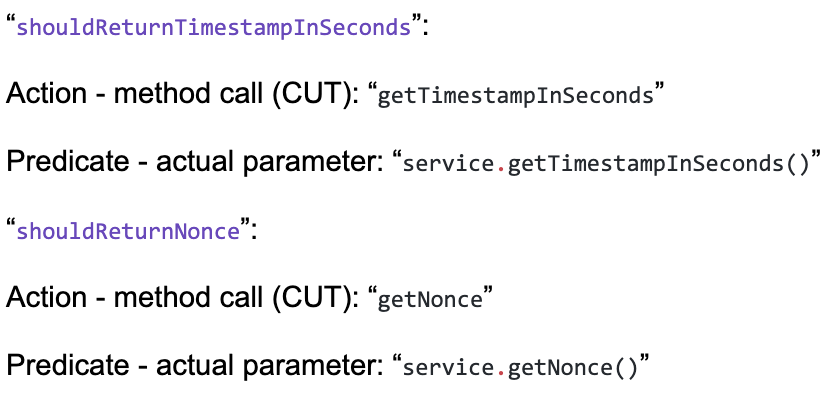
\includegraphics[scale=0.45]{figures/sp1-proposal.png}
\caption{Test cases with tagged text from the \enquote{Scribejava} project.}
\label{fig:test1-proposal}
\end{figure}

\begin{figure}[t]
\centering
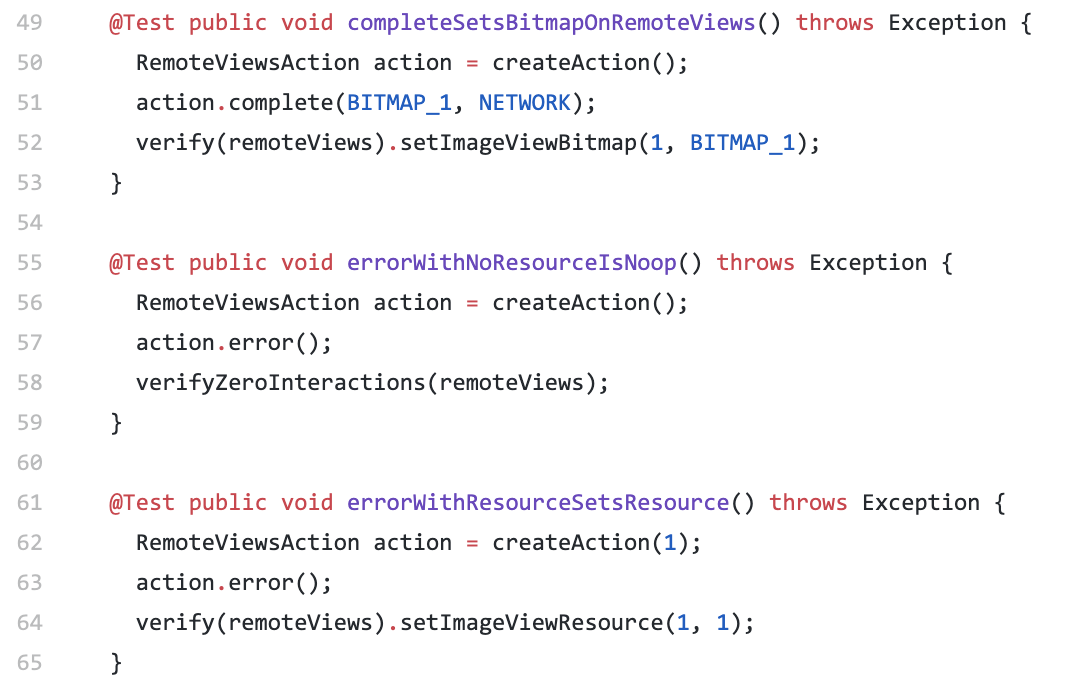
\includegraphics[scale=0.45]{figures/sp4-proposal.png}
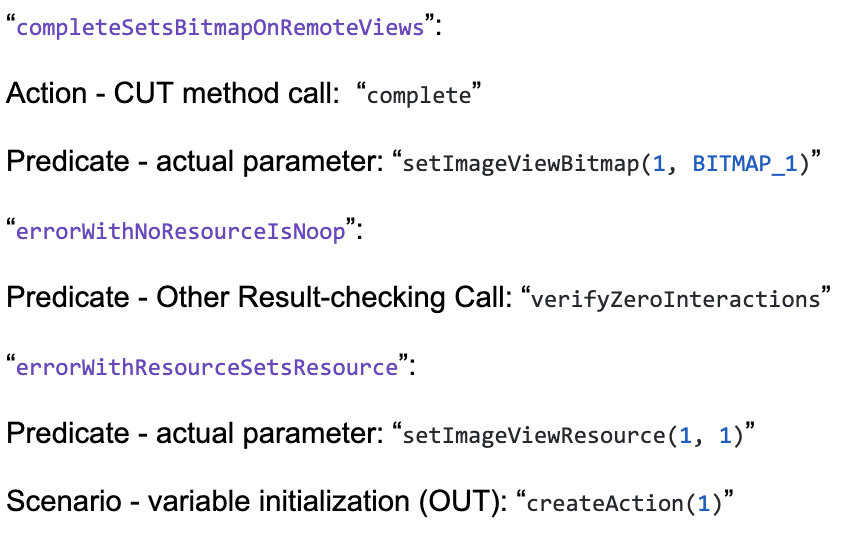
\includegraphics[scale=0.45]{figures/sp2-proposal.png}
\caption{Test cases with tagged text from the \enquote{Picasso} project.}
\label{fig:test2-proposal}
\end{figure}

\subparagraph{Combination}

The Combination code is applied to a test when none of the other top-level codes is applicable (i.e., the test’s action, predicate, and scenario are shared with other tests).
%
The secondary codes for the Combination code enumerate the possible combinations of the first three top-level codes: Action and Predicate, Action and Scenario, Scenario and Predicate; Action, Scenario, and Predicate.
%
For example, the Action and Predicate code will be applied when the action and predicate of the tests are not unique on their own but the combination of both of them is unique among other tests in the same test class.
%
The rest of the secondary codes of the Combination code follow the same pattern. The tagged text of each secondary code of the Combination code will be the structure of the combination, such as action and predicate or action and scenario.


\paragraph{Coding Process}

Using the selective codes and guidelines described above, each author individually recoded all of the \num{440} tests.
%
This was more straightforward than the initial open coding process because we were now familiar with the test and the results of the open and axial coding processes were already available.
%
Each test was first assigned one of more of the four top-level codes.
%
Then, for each top-level code that was assigned, one or more of the associated secondary-codes were assigned.
%
Again, after each author coded each test individually, the authors together examined the tagged tests in order to discuss and address any disagreements in the results.
%
At the end of this coding process we created a topical concordance that shows, for each code, the tests that have the corresponding type of uniqueness.
%
For the \num{440} tests that were selected from \num{11} projects, all the tagged results are shown in the online document~\cite{emp-study}.

As an example of the selective coding process, consider the examples in~\cref{fig:test1-proposal,fig:test2-proposal}.
%
The top-half of each figure shows an excerpt of a test class from one of the subjects considered in the study.
%
Note that some minor reformatting has been done to improve the presentation (i.e., all spaces and comments are removed).
%
The bottom of each figure shows the codes applied to each test using the format: $\langle top~level~code \rangle - \langle secondary~code \rangle$: \enquote{$\langle tagged~text \rangle $} where $\langle tagged~text \rangle $ shows the portion of the test body that is tagged by the secondary code.

% TODO [fixed]: Format all test names using \texttt and adding \- so they are hypehnated correctly.
For example in~\cref{fig:test1-proposal}, the test \texttt{should\-Return\-Timestamp\-In\-Seconds} is tagged with Action - method call (CUT): \enquote{\texttt{getTimestampInSeconds}} because no sibling shares the test’s action, which is to call the service’s timestamp functionality (i.e., the CUT Method \enquote{\texttt{getTimestampInSeconds()}}).
%
This test is also tagged with Predicate - actual parameter: \enquote{\texttt{service.getTimestampInSeconds()}} because no sibling test uses the result of calling \enquote{\texttt{getTimestampInSeconds}} as the actual parameter to an assertion method.
%
The test \texttt{should\-Return\-Nonce} is tagged with Action - CUT method call: \enquote{\texttt{getNonce}} because no sibling shares the test’s action, which is to call the service’s nonce functionality (i.e., the CUT Method \enquote{\texttt{getNonce()}}).
%
This test is also tagged with Predicate - actual parameter: \enquote{\texttt{service.getNonce()}} because no sibling test uses the result of calling \texttt{getNonce} as the actual parameter to an assertion method.


\begin{table*}[t]
\centering
\caption{Data of the top-level codes.\strut}
\begin{tabular}
{
  l
  S[table-format=5]
  S[table-format=5]
  S[table-format=5]
  S[table-format=5]
}
\toprule
\multicolumn{1}{c}{\textbf{Project}} &
\multicolumn{1}{c}{\textbf{Action}} & 
\multicolumn{1}{c}{\textbf{Predicate}} &
\multicolumn{1}{c}{\textbf{Scenario}} &
\multicolumn{1}{c}{\textbf{Combination}}
\\
 \midrule
 Barbecue          & 31  &  31   & 5     &  3 \\
 Guice             & 27  &  21   & 11    &  2 \\
 Mockito           & 23  &  25   & 18    &  3 \\
 Guava             & 20  &  19   & 11    &  5 \\
 Guice             & 23  &  23   & 24    &  1 \\
 ExoPlayer         & 26  &  21   & 10    &  4 \\
 Scribejava        & 30  &  17   & 15    &  2 \\
 Socket.io-client  & 28  &  15   & 14    &  4 \\
 Fastjson          & 30  &  26   & 7     &  3 \\
 picasso           & 16  &  24   & 10    &  2 \\
 Javapoet          & 17  &  35   & 3     &  4 \\
 \midrule
 \textbf{Sum}      & 271 &  257  & 128   &  33 \\
\bottomrule
\end{tabular}
\label{tab:top-level-codes}
\end{table*}

\begin{table*}[t]
\centering
\caption{Data for of the secondary codes.}
    \begin{subtable}[t]{1\textwidth}
    \centering
    \subcaption{Secondary codes for the Action code.}
    \begin{tabular}
    {
      l
      S[table-format=5]
      S[table-format=5.1]
    }
    \toprule
    \multicolumn{1}{c}{\textbf{Secondary Code}} &
    \multicolumn{1}{c}{\textbf{Frequency}} & 
    \multicolumn{1}{c}{\textbf{Percentage \%}}
    \\
    \midrule
     CUT call arguments     & 123  &  45.4  \\
     CUT method call        & 77   &  28.4  \\
     Other call arguments   & 44   &  16.2  \\
     Other method call      & 27   &  10.0  \\
    \bottomrule
    \end{tabular}
    \label{tab:secondary-codes-action}
    \end{subtable}
    \hfill \vspace{0.05cm}
    \begin{subtable}[t]{1\textwidth}
    \centering
    \caption{Secondary codes for the Predicate code.}
    \begin{tabular}
    {
      l
      S[table-format=5]
      S[table-format=5.1]
    }
    \toprule
    \multicolumn{1}{c}{\textbf{Secondary Code}} &
    \multicolumn{1}{c}{\textbf{Frequency}} & 
    \multicolumn{1}{c}{\textbf{Percentage \%}}
    \\
    \midrule
     Actual Parameter                & 134  &  52.1  \\
     Expected Parameter              & 78   &  30.4  \\
     Actual and Expected Parameters  & 26   &  10.1  \\
     Assertion Call                  & 18   &  7.0  \\
     Other Result-checking Call      & 1    &  0.4  \\
    \bottomrule
    \end{tabular}
    \label{tab:secondary-codes-predicate}
    \end{subtable}
    \hfill \vspace{0.05cm}
    \begin{subtable}[t]{1\textwidth}
    \centering
    \caption{Secondary codes for the Scenario code.}
    \begin{tabular}
    {
      l
      S[table-format=5]
      S[table-format=5.1]
    }
    \toprule
    \multicolumn{1}{c}{\textbf{Secondary Code}} &
    \multicolumn{1}{c}{\textbf{Frequency}} & 
    \multicolumn{1}{c}{\textbf{Percentage \%}}
    \\
    \midrule
     OUT Variable Initialization    & 94  &  73.4  \\
     Non-OUT Variable Initialization & 25   &  19.5  \\
     Non-OUT (other) Variable Initialization Arguments & 5 & 4.0  \\
     State-changing CUT Method Call       & 3   &  2.3  \\
     Control Flow Variable      & 1    &  0.8  \\
    \bottomrule
    \end{tabular}
    \label{tab:secondary-codes-scenario}
    \end{subtable}
    \hfill \vspace{0.05cm}
    \begin{subtable}[t]{1\textwidth}
    \centering
    \caption{Secondary codes for the Combination code.}
    \begin{tabular}
    {
      l
      S[table-format=5]
      S[table-format=5.1]
    }
    \toprule
    \multicolumn{1}{c}{\textbf{Secondary Code}} &
    \multicolumn{1}{c}{\textbf{Frequency}} & 
    \multicolumn{1}{c}{\textbf{Percentage \%}}
    \\
    \midrule
     action+scenario+predicate & 15   &  45.5  \\
     scenario+predicate        & 11   &  33.3  \\
     action+predicate          & 4    &  12.1  \\
     action+scenario           & 3    &  9.1  \\
    \bottomrule
    \end{tabular}
    \label{tab:secondary-codes-combination}
    \end{subtable}
\label{tab:secondary-codes}
\end{table*}


In~\cref{fig:test2-proposal}, the test \texttt{complete\-Sets\-Bitmap\-On\-Remote\-Views} is tagged with Action - CUT method call: \enquote{\texttt{complete}} because no sibling shares the test’s action, which is to call a method to the action’s complete functionality (i.e., the CUT Method \enquote{\texttt{complete()}}).
%
This test is also tagged with Predicate - actual parameter: \enquote{\texttt{setImageViewBitmap(1, BITMAP\_1)}} because no sibling test utilizes the \texttt{setImageViewBitmap(1, BITMAP\_1)} as the actual parameter in an assertion.
%
The test \texttt{error\-With\-No\-Resource\-Is\-Noop} is tagged with Predicate - other result-checking call: \enquote{\texttt{verifyZeroInteractions}} because no sibling shares the test’s predicate, which is to call a verification method \texttt{verifyZeroInteractions} to check the behavior of the \texttt{remoteViews} variable.
%
The test \texttt{error\-With\-Resource\-Sets\-Resource} is tagged with Predicate - actual parameter: \enquote{\texttt{setImageViewResource(1, 1)}} because no sibling shares the test’s predicate, which is to verify the behavior of \texttt{remoteViews} variable with a specific parameter and utilizes the \texttt{setImageViewResource(1, 1)} as the actual parameter in an assertion.
%
This test is also tagged with Scenario - variable initialization (OUT): \enquote{\texttt{createAction(1)}} because no sibling shares the test’s scenario because no other test initializes the \enquote{action} variable (i.e., the object under test) using the \texttt{createAction(1)} as its variable initialization.


To better understand the results of the coding process we gathered some descriptive statistics.

\Cref{tab:top-level-codes} shows the frequency of the top-level codes across the sampled tests.
%
In this table, the first column, Project, shows the name of the subject and the following four columns, Action through Combination, show the number of times each top-level code was applied to tests from the corresponding subject.
%
For example, the first row shows that, for the tests sampled from Barbecue, the Action code was applied \num{31} times, the Predicate code was applied \num{31} times, the Scenario code was applied \num{5} times, and the Combination code was applied \num{3} times.
%
The final row in the table shows how many times each code was applied across all tests.

\Cref{tab:secondary-codes-action,tab:secondary-codes-predicate,tab:secondary-codes-scenario,tab:secondary-codes-combination} show the frequencies of each secondary code.
%
In each table, the first column, Secondary Code, shows the secondary codes; the second column, Frequency, shows the number of times each secondary code was applied across all projects; and the final column, Percentage, shows how often the secondary code was applied, given its associated top-level code.
%
For example, the second row in~\cref{tab:secondary-codes-action} shows that the secondary code \enquote{CUT method call} was applied \num{77} times which is approximately \SI{\approx 28}{\percent} of the \num{271} times the top-level Action code was applied (i.e., when it was possible to apply the secondary code).

Based on the data shown in these tables, we can draw some general observations.
%
The first observation is about the relative frequencies of the top level codes: the Action and Predicate codes are the most common and occur about the same amount of the time (\num{271} out of \num{689}, \SI{\approx 39}{\percent} and \num{257} out of \num{689}, \SI{\approx 37}{\percent}, respectively); the Scenario code is less common (\num{128} out of \num{689}, \SI{\approx 19}{\percent}); and the Combination code is the least common and is relatively rare (\num{33} out of \num{689}, \SI{\approx 5}{\percent}).
%
This suggests that there is often a single part of a test that makes it unique among its siblings and the action and predicate are what makes it unique most often.
%
The second observation is that the relative frequencies of the top level codes within each project is largely consistent with the overall distribution.
%
With the exception of Guice, the Combination code is always the least common and the Scenario code is the second least common.
%
This suggests that the relative frequencies are likely to hold across most projects.
%
The final observation is about the relative frequencies of the secondary codes.  With the exception of the OUT Variable Initialization secondary code (\num{94} out of \num{128}, \SI{\approx 73}{\percent}), there are no dominant secondary codes (e.g., \SI{> 70}{\percent}).
%
This suggests that while there may be trends among the part of a test that makes it unique (e.g., action, scenario, and predicate), the specifics of what make each of these parts of the test unique varies greatly.
%
In addition, with the exception of Javapoet (which relies on the secondary codes under the predicate top-level code, 35 out of 59, \SI{\approx 60}{\percent}), there are also no dominant secondary codes (e.g., \SI{>= 60}{\percent}) at the project level, and the rest of the detailed data can be found in the online document~\cite{emp-study}.


\subsubsection{Results and Discussion}

\begin{table}[t]
\centering
\caption{Results to check if the tokens are identical or transformed.\strut}
\small
\begin{tabular}
{
  l
  S[table-format=5]
  S[table-format=5]
  S[table-format=5]
  S[table-format=5]
  S[table-format=5]
  S[table-format=5]
  S[table-format=5]
}
\toprule
\multicolumn{1}{c}{\textbf{Project}} & \multicolumn{3}{c}{\textbf{Full}} & \multicolumn{3}{c}{\textbf{Partial}} & \multicolumn{1}{c}{\textbf{None}}\\
\cmidrule(lr){2-4}
\cmidrule(lr){5-7}
\cmidrule(lr){8-8}

& \multicolumn{1}{c}{\textbf{\# Tests}} & \multicolumn{1}{c}{\textbf{Identical}} & 
\multicolumn{1}{c}{\textbf{Transformed}} &
\multicolumn{1}{c}{\textbf{\# Tests}} &
\multicolumn{1}{c}{\textbf{Identical}} &
\multicolumn{1}{c}{\textbf{Transformed}} &
\multicolumn{1}{c}{\textbf{\# Tests}}
\\
\midrule
 Barbecue           & 2  &  0  & 2   & 32 & 27 & 5 & 6 \\
 Moshi              & 5 &  5  & 0   & 18 & 16 & 2 & 17 \\
 Mockito            & 4  &  3  & 1   & 27 & 24 & 3 & 9 \\
 Guava              & 2  &  2  & 0  & 30 & 27 & 3 & 8 \\
 Guice              & 1  &  1  & 0   & 36 & 29 & 7 & 3 \\
 ExoPlayer          & 3  &  3  & 0  & 19 & 16 & 3 & 18 \\
 Scribejava         & 5  &  5  & 0  & 31 & 28 & 3 & 4 \\
 Socket.io-client   & 0  &  0  & 0  & 36 & 22 & 14 & 4 \\
 Fastjson           & 1  &  1  & 0   & 20 & 19 & 1 & 19 \\
 Picasso            & 2  &  2  & 0   & 29 & 25 & 4 & 9 \\
 Javapoet           & 0  &  0  & 0   & 31 & 28 & 3 & 9 \\
 \midrule
 Overall            & 25 &  22  &  3  & 309 & 261 & 48 & 106 \\
\bottomrule
\end{tabular}
\label{tab:identical-or-transformed}
\end{table}

The goal of the second part of our study is to investigate whether tests are named, either wholly or in part, after what makes them unique.
%
In order to decide whether tests are named after what makes them unique, we investigated two research questions:
\begin{itemize}
    \item RQ1: Is uniqueness used as a naming rationale for JUnit tests?
    \item RQ2: When uniqueness is the naming rationale, does the tagged text appear directly in the name or is it transformed?
\end{itemize}

\paragraph{RQ1: Is uniqueness used as a naming rationale in JUnit tests?}

To investigate RQ1, we manually compared the name of each test against the aspects that make it unique which were identified in the first part of the study.
%
The comparison between the test name and tagged text (i.e.,the aspects of the test that make it unique) is performed as follows.
%
First, we manually split the test names and the tagged text into a set of tokens using a customized tokenizer for identifiers~\cite{enslen2009mining}.
%
Then we lower case all tokens and remove a leading \enquote{test}, as well as connectors that are rarely used in the test body (e.g., not, to, then, etc.).
%
For example, the test name \texttt{test\-Post\-Returns\-Barcode\-Image} is parsed into a set of tokens:~$\langle post,~returns,~barcode,~image \rangle$.
%
Finally, we manually compared the two sets of tokens.
%
Each author did this comparison individually and classified the tests into one of the following categories based on the degree to which the name appears to be based on the tagged text.

\begin{enumerate}

\item Full: The tests in the Full category appear to be named wholly after what makes the test unique (i.e., every token from the name appears to be derived from a token from the tagged text).
%
For example, for \texttt{test\-Put\-All} from Guava, the tokens from the name are $\langle put,~all \rangle$ and the tokens from the tagged text are also $\langle put,~all \rangle$.
%
Because each token in the token set of the name originates from a corresponding token from the token set of the tagged text (e.g., both tokens are literally the same or share the same meaning), \texttt{test\-Put\-All} is included in the Full category.
%
As another example, consider \texttt{test\_geo} from FastJson.
%
For this test, the tokens from the name are $\langle geo \rangle$ and the tokens from the tagged text are $\langle geometry \rangle$.
%
Because \enquote{geo} appears to be an abbreviation for \enquote{geometry}, each token from the name is derived from a token from the tagged text and the test is also included in the Full category.

\item Partial: The tests in the Partial category appear to be named partially after what makes the test unique (i.e., at least one token from the name appears to be derived from a token in the tagged text).
%
For example for \texttt{test\-Checksum\-Is\-Null} from Barbecue, the tokens from the name are $\langle checksum,~is,~null \rangle$ and the tokens from the tagged text are $\langle calculate,~checksum \rangle$.
%
Because the token \enquote{checksum} in the token set of the test name is directly derived from the token \enquote{checksum} in the token set of the tagged text, \texttt{test\-Checksum\-Is\-Null} is included in the Partial category.
%
As another example, consider \texttt{test\-Child\-Bindings\-Not\-Visible\-To\-Parent} from Guice, the tokens from the test name are $\langle child,~bindings,~visible,~parent \rangle$ and the tokens from the tagged text are $\langle get,~binding \rangle$.
%
Because the token \enquote{bindings} from the test name is the plural of the token \enquote{binding} from the tagged text, \texttt{test\-Child\-Bindings\-Not\-Visible\-To\-Parent} is also included in the Partial category.

\item None: The tests in the None category do not appear to be named after what makes the test unique (i.e., none of the tokens from the name appear to be derived from a token from the tagged text).
%
For example, for \texttt{test\-Value\-Is\-Required} from Barbecue, the tokens from the test name are $\langle value,~is,~required \rangle$ and the tokens from the tagged text are $\langle remove,~servlet,~exception \rangle$.
%
Because none of the tokens from the test name appears to be derived from the tokens from the tagged text, \texttt{test\-Value\-Is\-Required} is listed in the None category.
\end{enumerate}

Again, after each author classified each test individually, the authors together examined the classification in order to resolve any disagreements.
%
The results of the rectified classification are shown in~\Cref{tab:identical-or-transformed}.
%
In the table, the first column, \emph{Project}, shows the name of each project and the subsequent three columns, \emph{Full}, \emph{Partial}, and \emph{None}, show the number of tests in each category, respectively.
%
The first sub-column, \emph{\# Tests}, indicates the total number of tests that is under each main category and the other two sub-columns, \emph{Identical} and \emph{Transformed}, will be explained later.
%
For example, the first row shows the data collected from Barbecue: a total of \num{2} tests are in the Full category, a total of \num{32} tests are in the Partial category, and a total of \num{6} tests are in the None category (i.e., sum to \num{40} per project).
%
Finally, the last row shows the totals for each category across all inspected projects.


As the data in~\Cref{tab:identical-or-transformed} shows, most of the tests (\num{334} out of \num{440}, \SI{\approx 76}{\percent}) are in either the Full or the Partial category, and Partial is the majority of these two categories.
%
However, there are also a significant fraction of tests in the None category (\num{106} out of \num{440}, \SI{\approx 24}{\percent}).
%
We found this surprising, especially considering that tests with bad names were excluded from our set of tests.
%
To better understand the causes behind this, we further investigated the tests in this category.
%
We found that while these test names are not based on what makes the test unique, they do often follow a reasonable naming rationale.
%
The most common rationale (\num{34} out of \num{106}, \SI{\approx 32}{\percent}) is because a number of tests are named after something that is out of the scope of their current test bodies, which could be derived from a setup of the testing environment, a implicit behavior of the program, or even a combined naming scheme of different sources.
%
For example, \texttt{test\-Value\-Is\-Required} from Barbecue is designed to make sure when there is a missing value in the required parameters of the setup of its test class, an exception will be thrown and caught.
%
However, the setup of the test class is clearly out of the scope of a single unit test. 


The second most common rationale in the tie is due to that some tests were written in the acceptance testing phase to mimic a certain behavior of the actual user, which is less common than the first rationale (\num{30} out of \num{106}, \SI{\approx 28}{\percent}).
%
For example, \texttt{load\-Throws\-With\-Invalid\-Input} from Picasso is designed to make sure that when the user enters an invalid input (i.e., URL for this test), a corresponding exception must be thrown.
%
The third most common rationale (\num{29} out of \num{106}, \SI{\approx 27}{\percent}) is owing to the fact that some tests are named after something from their test bodies but it is not what makes those tests unique.
%
For example, \texttt{test\-Read\-Full} from Exoplayer is designed to check if a specific data source can be fully read. This test is named after the CUT method call $\langle read \rangle$, nevertheless this call is used by other tests in the same class for multiple times.
%
Overall, about \SI{88} of the tests under the none category are named using a different rationale. 
%
The remaining tests (\num{13} out of \num{106}, \SI{\approx 12}{\percent}) were tests with poor names that were not caught by our conservative filtering.
%
For example, JavaPoet contains a test named \enquote{usage} that does not provide any useful information about how the \enquote{usage} is related to the content of the test.
%
In our planned future work, we will introduce another technique to handle those three types of names, but it is not the current focus of this paper.
%
The detailed data is shown in the shared document~\cite{emp-data}.


Based on the data in~\Cref{tab:identical-or-transformed} and our additional investigation of tests in the None category, we conclude that the answer to RQ1 is \enquote{yes}.
%
Uniqueness is indeed commonly used as a naming rationale when constructing the names of JUnit tests.
%
From the \num{440} selected tests, most of them are named under the uniqueness-based naming rationale, and their test names at least partially reflect the uniqueness by containing some or all of the tokens from the tagged text.


\paragraph{RQ2: When uniqueness is the naming rationale, does the tagged text appear directly in the name or is it somehow transformed?}

To gain some additional insights in to how much extra work an automated tool might need, we further examined the tests in the Full and Partial categories to determine whether the information about what makes the test unique has the same form in the name or if it was transformed in some way.
%
In order to get the information from the collected data, we performed a manual classification of all the tests in the full and partial categories.
%
In this case were classified the tests as either Identical or Transformed.

\begin{enumerate}
\item Identical: The tests in the Identical sub-category have this feature: each token from the test name that appears to come from the tagged text is identical to the token from the tagged text.
%
For example, for \texttt{should\-Include\-Port8080} from Scribejava, the tokens from the name are $\langle should,~include,~port8080 \rangle$ from the name, and tokens from the tagged text are $\langle request,~port8080 \rangle$.
%
The token \texttt{port8080} from the tokens of the name appears to come from the token \texttt{port8080} from the tokens of the tagged text, and they are identical to each other, so \texttt{should\-Include\-Port8080} is included in the Identical category.

\item Transformed: The tests in the Transformed sub-category have this feature: each token from the test name that appears to come from the tagged text is transformed to the token from the tagged text, and it often indicates that both tokens from the name and tagged text have the same meaning but in different forms (i.e., abbreviation, plural and singular form, etc.).
%
For example, for \texttt{should\-Return\-Url\-Param} from Scribejava, the tokens from the name are $\langle should,~return,~url,~param \rangle$, and the tokens from the tagged text are $\langle get,~parameter,~null,~access,~secret \rangle$.
%
The token \enquote{param} from the name appears to come from the token \enquote{parameter} from the tagged text, and it is a transformation of the token \enquote{parameter} from the tagged text by using the abbreviation of the word.
\end{enumerate}


The results of this additional classification are also shown in~\Cref{tab:identical-or-transformed}.
%
The Identical and Transformed sub-columns show the number of tests with their names in the identical and transformed categories, respectively.
%
For example, the data from the third row shows the project Mockito has \num{4} tests that are fully named after the tokens from the tagged text.
%
Of these \num{4} test names, \num{3} of them are under the Identical category, which indicates each of them has a shared subset of tokens between the tokens from its name and the tagged text.
%
Each token in the shared subset is identical when comparing between the name and the tagged text (i.e., a physical intersection exists between the two sets of tokens from the name and the tagged text).
%
\num{1} of them is under the Transformed category, and this test also has a shared subset of tokens between the tokens from its name and the tagged text.
%
Differently, each token in the shared subset is transformed from its appearance in the tokens of the name to its corresponding appearance in the token of the tagged text (i.e., a conceptual intersection exists between the two sets of tokens from the name and the tagged text).

Moreover, it also shows Mockito has \num{27} tests that are partially named after the tokens from the tagged text.
%
Of these \num{27} test names, \num{24} of them have the identical tokens between the name and the tagged text, and \num{3} of them has the same tokens between the name and the tagged text but the tokens of the name are transformed from the tokens of the tagged text.
%
At the end, there are \num{9} tests in Mockito that are not named after the tokens from the tagged text at all.
%
The data for each project slightly varies from each other, but the distribution of the identical and transformed tokens are largely consistent.
%
For example in~\Cref{tab:identical-or-transformed}, the number of identical tokens for each project is usually greater than the number of transformed tokens, and the majority of tokens from the name are identical to those from the tagged text (i.e., \num{22} out of \num{25} for full, and \num{261} out of \num{309} for partial).
%
Therefore, RQ2 is answered with \enquote{yes} and \enquote{both} since both the identical and the transformed tokens were found in the comparison between the tokens from the name and the tagged text.

Judging from the results of both RQ1 and RQ2, the majority of the test names are indeed named after the tokens from the tagged text, and the tokens between the name and tagged text are mostly identical to each other, so we decided to proceed to build the automated tool.



\subsubsection{Remaining Work: Implementation and Evaluation of the Concept-based Approach}
\label{sec:remaining-work}

In my preliminary work, I built a pattern-based approach to detect and improve non-descriptive test names.
%
However, the pattern-based approach is limited to one perspective of the solving the naming problem for unit tests that is to improve test names with descriptiveness, but the uniqueness of tests is not mentioned in this work.
%
Especially, pattern mining in the pattern-based approach requires close attention to each component of every test pattern, which is both difficult and labor intensive.
%
In the remaining work, I plan to develop a concept-based approach that uses a set of top-level and secondary codes produced by the selective coding in the empirical study for tagging and extracting the uniqueness from the tests.
%
First, using the set of top-level and secondary codes that were previously selected, it is feasible for us to build a concept-based approach to check and improve existing test names with a uniqueness-based naming rationale.
%
Second, after the concept-based approach is completed, an empirical evaluation is also needed to further investigate the correctness, effectiveness, and comprehensibility of the approach.
%
As mentioned in~\cref{sec:introduction}, the goal of my proposed research is to systematically provide descriptive and unique test names, so there are still several attributes of test names that can be explored.
%
Therefore, for the last aspect of test names, I plan to consider the naming problem of unit tests from another innovative aspect, which is to build a shape-based approach that learn from how different shapes of a test name (i.e., length, camel cases, underscores, descriptiveness, uniqueness) affect developers' understanding of the corresponding tests.

\subsubsection{Implementation of the Concept-based Approach}

Utilizing the top-level and secondary codes that were created in the empirical study section~\cref{sec:empStudy}, the next step is to build a concept-based approach that can improve existing test names by a uniqueness-based naming rationale for developers.
%
For the implementation, I plan to introduce the idea of formal concept analysis (FCA) as the main method, and how to integrate it with the top-level and secondary codes will also be explained.
%
Using the implicit relationships extracted by FCA and the existing codes, a concept-based approach can not only correctly tag the codes to the tests but also provide a uniqueness-based naming rationale for improving the existing test names.

\subsubsection{Evaluation of the Concept-based Approach}

Research questions involved in this step are:
%
\begin{enumerate}
    \item RQ1-Correctness: Can the concept-based approach apply the top-level and secondary codes to each test correctly?
    \item RQ2-Effectiveness: Does the tagged text of each test accurately describe the uniqueness of the test?
    \item RQ3-Comprehensibility: Is the generated results of the concept-based approach straightforward enough to be easily understood?
\end{enumerate}.

For answering RQ1, I plan to perform a quantitative analysis by comparing the results from manual tagging of a randomly set of tests (i.e., from 5 random Java projects on Github) with the results from the concept-based approach to see if the two different results are matched.
%
For answering RQ2, I plan to further check if the tagged text that was generated by the concept-based approach is the same as the tagged text from the manual tagging from the same set of tests.
%
For answering RQ3, I plan to conduct a small scale survey that 4 experienced developer will participate, and several survey questions about if they can easily understand and apply the results from running the concept-based approach will be presented to the participants.




\section{Foreseen Contributions}
\label{sec:contributions}

\textbf{---To be changed---}

In this proposal, I propose three research directions that focus on systematically providing descriptive and unique names for unit tests.
%
In the preliminary work, first, an empirical study to investigate if unit tests are named after what makes them unique was conducted to motivate all the following work.
%
Besides the preliminary work, I first plan to use the results from the empirical study to develop a concept-based approach that provides a uniqueness-based naming rationale for unit tests.
%
Then I plan to develop a pattern-based approach that can detect and improve non-descriptive test names, which is already completed in the preliminary work.
%
The empirical study and the pattern-based approach combine pattern mining, static program analysis, NLPA, selective coding, and quantitative analysis.
%
Secondly, I plan to create a shape-based approach that can measure if the physical appearance (i.e., length, camel case, etc.), descriptiveness, and uniqueness of test names can affect how developers understand those tests by using a eye-tracking method.

The following list presents a summary of my contributions:
\begin{enumerate}
    \item a novel, concept-based approach that can check if a test is named after what makes it unique and help developers improve existing test names with uniqueness
    \item a new, pattern-based approach that can detect and improve non-descriptive test names
    \item an innovative, shape-based approach that can measure if the physical appearance, descriptiveness, and uniqueness of test names can affect how developers understand those tests.
\end{enumerate}.

I anticipate that my research can systematically help test developers to identify and improve existing test names with three different types of descriptiveness that provide the summarized information from the test body.
%
At the same time, quality and maintainability of unit tests could be significantly improved by using my approaches.

\section{Related Work}
\label{sec:related-work}

Existing work related to my proposed research will be discussed in this section. I have organized them into the following categories:

\subsection{Detecting Mismatches\slash Improving Names}


There are some existing works that attempt to identify name\slash implementation mismatches.

\Citeauthor{host2009debugging}'s work is the most similar to our approach as it attempts to identify several types of naming bugs in general Java methods~\cite{host2009debugging}.
%
Their approach relies on a manually generated rule book that is extracted from the implicit convention between names and implementations in Java programming, which can be utilized to detect name bugs and provide some suggestions for constructing more suitable names.
%
In their previous works, \citeauthor{host2008java} already showed that there is a mutual dependency between method names and their associated implementations~\cite{host2008java}.
%
Therefore, their approach considered the mismatch between the name and the implementation of its associated method and used the mismatch to fix name bugs, which are both similar to the analytical process and goal of our pattern-based approach.
%
There are two major differences between their work and ours.
%
First, our approach primarily focuses on the test names rather than general method names that often follow a different naming convention.
%
For example, their approach treated the data type of the value in the \texttt{return} statement as an essential attribute in their rule book.
%
However, normally for the unit tests, they compared different values using the \texttt{assertions} rather than any \texttt{return} statement, so the information in those \texttt{assertions} will be a crucial part of their test names.
%
Second, instead of using a manually generated rule book, we built our approach based on the test patterns, and those test patterns were mined from a large test corpus by a semi-automatic process.

% TODO->[fixed, moved allamanis2015suggesting&daka2017generating to next section]: Are't some of these works more approach for generating names from scratch rahter than suggesting improvemnts?
\citeauthor{zhong2013detecting} provided a novel approach for detecting API documentation errors, and those errors are essentially the mismatches between the API documentation and the actual programs~\cite{zhong2013detecting}.
%
To address the importance of words in Java programming, \citeauthor{singer2008exploiting} showed that words in class names are closely related to class properties that can be described in micro patterns~\cite{singer2008exploiting}.
%
\citeauthor{allamanis2014learning} mentioned that developers should follow a consistent naming convention, and they proposed a novel framework that can suggest identifier names accurately~\cite{allamanis2014learning}.
%
All of their works comprehensively showed it is feasible to find poorly structured (i.e., non-descriptive) names by using the mismatch or pattern between the name and the program, and we can also improve those names by using providing accurate suggestions.
%
Nonetheless, each of their techniques is often limited to a certain aspect in the problem of detecting and improving non-descriptive names, so none of them can be directly applied to improving non-descriptive names in unit tests.
%
\citeauthor{pradel2018deepbugs} recently proposed a framework for the detection of naming bugs~\cite{pradel2018deepbugs}.
%
Regardless of their effort to introduce a new approach that can detect name-based bugs by using their machine learning method, we still can not apply their approach to the unit tests without further modifications.
%
Because some unit tests are expected to produce certain exceptions or failures when using them, so testers might intentionally design poorly named identifiers in those tests.
%
Consequently, lots of false-positives could be generated without a complete retrofit to extend their proposed framework to unit tests.
% change done ->
For instance, Junit 4 requires every test name to have a leading \enquote{test} \cite{JUnit4}, so some of existing techniques might consider the leading \enquote{test} as the action, predicate, or scenario of the name.


\subsection{Automated Generation of Test Names}

In contrast to the techniques mentioned above that attempt to improve names, there are several approaches that attempt to automatically generate names.
%
Some of these techniques use natural language-based program analysis~(NLPA).
%
For example, \citeauthor{zhang2016towards} proposed their approach that can generate descriptive names from existing test bodies by using natural-language program analysis and text generation~\cite{zhang2016towards}.
%
However, their approach left an important question unanswered that is testers need to decide which one of the three possible test names should be used for their unit tests by themselves, and it is possible that none of the three generated names follow the common naming convention.
%
Other techniques utilized Java bytecode, method-call sequences, API-level coverage goals, and \texttt{logbilinear} context models~\cite{fraser2011evosuite,thummalapenta2009mseqgen,daka2017generating,allamanis2015suggesting}.
%
Even with their automated generation process, their generated test names are not human-readable that can cause misunderstanding for testers who want to further modify those generated test names or bodies.
% change done ->
Although some techniques can generate descriptive names, those techniques required testers to perform a full test execution with certain coverage goals or building a context model, which are often error-prone in practice (i.e., those coverage goals or models might be too specific to apply for certain projects).

Recent work tried to solve the naming problem of unit tests by using machine learning-based approaches~\cite{alon2018code2seq, alon2019code2vec}.
%
Although using machine learning-based models can accurately summarize the important information from the test body, their predicted test names often do not fit developer need that is to be unique among its siblings.
%
To understand how limited these machine learning-based approaches are, we conducted a pilot study with a set of \num{11} randomly selected projects (i.e., contain \num{25567} unit tests) that contain a complete suite of JUnit tests.
%
The \num{11} Java projects are built for various purposes like Guava is an open-source common library for Java and fastjson is a JSON parser\slash generator.

If many generated test names are repeated at least once in its associated test class and there are lots of duplicated names during the name generation process, it is then necessary to develop a uniqueness-focused approach.
%
In order to measure the level of duplication, we performed a quantitative analysis on the collected result.
%
The data of the quantitative analysis is shown in this shared document~\cite{CodeResult}, and it shows that hundreds or thousands of duplicate test names were generated for each project (i.e., either using~\cite{alon2018code2seq} or~\cite{alon2019code2vec}).
%
For example, \enquote{Code2seq} produced \num{80} repeating test names for the moshi project, and \num{14} out of \num{24} test classes in the moshi project contain more than one repeating test names.
%
For another example, \enquote{Code2vec} produced \num{1199} repeating test names for the guava project, and \num{211} out of \num{461} test classes in the guava project contain more than one repeating test names.
%
This observation during the quantitative analysis indicates there is a need to develop a uniqueness-based naming rationale that can be used to generate descriptive (i.e., being unique and informative) test names.


\subsection{General Program Analysis\slash Automated Testing and Debugging}

Many researchers proposed their program analysis or automated testing techniques that can help us have a better understanding of the embedded features in unit tests. 
%
\citeauthor{moreno2012jstereocode} proposed Java method and class stereotypes, and they took a closer look at the statement level analysis of Java code~\cite{moreno2012jstereocode}, and~\citeauthor{ghafari2015automatically} tried to extract the focal method under test~\cite{ghafari2015automatically}.
%
To be more focused on unit testing,~\citeauthor{li2018aiding} constructed a series of tags for distinguish unit test cases~\cite{li2018aiding}.
%
A group of researchers also conducted a series of works related to tagging methods or classes with stereotypes~\cite{dragan2006reverse,dragan2010automatic,dragan2011emergent}, but their works might also not be applicable for unit tests.
%
From a general perspective of testing, other researchers tried to devise methods that can perform fully automated testing by the targeted event sequence or the environmental dependencies~\cite{jensen2013automated,arcuri2014automated}.
%
All of their works performed well under their specific problems in program analysis or automated testing. 
% change done here
However, while their works focus more on extracting features from code or automating the testing process rather than the unit tests themselves, we can still use them to improve our pattern-based approach.
%
Furthermore, \citeauthor{li2019deepfl} proposed a learning-based approach for fault localization and automated debugging with high performance~\cite{li2019deepfl}, but the goal of their work is primarily to locate software faults for debugging rather than the naming of unit tests. 
%
Regardless of the performance of their proposed tool, the goal of their work is primarily to locate software faults for debugging rather than the naming of unit testing, and the experimental subjects they used is a standard benchmark database of detecting bugs rather than the unit tests from real-world Java projects.


\subsection{Natural Language Program Analysis}

There are lots of existing works that try to analyze programs from a natural language-based perspective.
%
\citeauthor{pollock2007introducing} and~\citeauthor{shepherd2007using} introduced NLPA by illustrating how to apply NLPA in practice and also giving some insights about aspect mining~\cite{pollock2007introducing,shepherd2007using,pollock2009natural}.
%
Their studies showed natural language clues from developers' naming style can be used for improving the effectiveness of software tools.
%
\citeauthor{abebe2010natural} proposed a natural language-based method to parse the identifier names of program elements for extracting concepts from them~\cite{abebe2010natural}.
%
Furthermore, some researchers attempted to split identifiers~\cite{enslen2009mining,butler2011improving,guerrouj2013tidier,hill2014empirical}, and others managed to expand abbreviations~\cite{hill2008amap,madani2010recognizing,corazza2012linsen}.
%
Even though their works are not alternatives to our approach, we can still use their implemented tools to improve the accuracy of the test patterns.


\subsection{Formal Concept Analysis}

As a well-developed technique for deriving a concept hierarchy from objects through a set of attributes, formal concept analysis (FCA) is an excellent method to use for analyzing data like the process of human thinking~\cite{ganter2012formal,yao2004comparative}.
%
Moreover, a early survey has already been conducted to discover the possibility of solving software engineering problem by using concept analysis~\cite{tilley2005survey}.
%
Many researchers focused on using FCA as an efficient method to provide solutions for various software engineering problems~\cite{godin2005formal,park2000software,cellier2008formal,hesse2005formal,mens2005delving}, and they used concept analysis to mock how human (i.e., developers) thinks about writing software or trace the thinking inside existing software.
%
However, none of them focused on applying FCA to unit tests, and their technique paid more attention to use FCA to understand the high-level structure of software rather than improving the naming in unit tests.

Other works also managed to utilize formal concept analysis as a method to resolve specific problems.
%
\citeauthor{he2011test} developed FCA-based technique for test case generation of mutation testing \cite{he2011test}.
%
\citeauthor{khor2004using} proposed a automatic test generator that uses formal concept analysis to manage the relationships between tests \cite{khor2004using}.
%
\citeauthor{cimiano2005learning} tried to extract concept hierarchies from text corpus by using their proposed techniques based on formal concept analysis \cite{cimiano2005learning}.
%
\citeauthor{tonella2004aspect} managed to perform aspect mining on execution traces by using formal concept analysis \cite{tonella2004aspect}.
%
However, all of their works focused on solving those specific problems, so their approaches might not be applicable for providing descriptive names for unit tests.


\subsection{Investigating Developer's Focus in Software Development}

In recent years, a novel study of tracking the eye movement of developers emerged in the effort to understand the behavior of developers in the process of software development.
%
\citeauthor{rodeghero2015empirical} conducted an empirical study to discover the patterns of eye movement when developers perform summarization tasks~\cite{rodeghero2015empirical}.
%
\citeauthor{begel2018eye} performed a pilot study of capturing the eye movements of multiple developers in the process of code review, which was inspiring for building a automated tool for code review~\cite{begel2018eye}.
%
\citeauthor{abid2019using} focused on building a mental cognition model to understand how developers understand codes~\cite{abid2019using}.
%
\citeauthor{obaidellah2018survey} conducted a throughout survey on the usage of the eye-tracking technology in the research of program comprehension~\cite{obaidellah2018survey}.
%
\citeauthor{abid2019developer} presented a eye-tracking study that shows the behavior of developers when summarizing Java methods~\cite{abid2019developer}.
%
\citeauthor{ioannou2020mining} proposed a series of reading pattern by mining the eye-tracking data for comprehending the behavior of developers~\cite{ioannou2020mining}.
%
All of the recent work provided a great insight for us to choose which of the code elements should be selected as the secondary codes and helped us to have a profound understanding of the focus of actual developers.
%
Nevertheless, their work primarily focused on the eye-tracking of developers when reading the general Java methods and classes, not unit tests.
%
Moreover, their work did provide some results from those eye-tracking studies, but no formal approach is proposed to detect and extract the unique coding of unit tests.




\bibliographystyle{abbrvnat}
\setlength{\bibsep}{2pt}
\newpage
\bibliography{proposal.bib}

\end{document}
